\documentclass[aspectratio=169,10pt]{beamer}
\usetheme{mekatronik}
\setday{5}{Resonance, Sensors, Measurement \& Integration}
\title[Day 5: Resonance, Sensors \& Integration]{Resonance, Sensors, Measurement and System Integration}
\subtitle{3.7 Resonance \& filters \textbullet\ 4.1 Sensors \textbullet\ 4.2 Encoders \& resolvers \textbullet\ 4.3 Sampling \textbullet\ 4.4 Signal processing \textbullet\ 4.5 Communication}
\author{Mechatronics Training Programme}
\institute{Theoretical Course Series}
\date{Day 5 of 5}

\pgfplotstableset{col sep=space}
\newcommand{\dat}[1]{data/#1.dat}
\tikzset{
  blk/.style={draw=mkBlue,fill=mkPale,thick,rounded corners=1pt,minimum height=7mm,minimum width=12mm,align=center,font=\scriptsize},
  sumn/.style={draw=mkBlue,fill=white,thick,circle,inner sep=0pt,minimum size=4.5mm},
  sig/.style={-{Latex[length=2mm]},thick,mkNavy},
  lbl/.style={font=\scriptsize,text=mkGray},
}

\newcommand{\lbx}[4]{\draw[thick,fill=#4] (#1,0) rectangle (#2,.6); \node[align=center] at ({(#1+#2)/2},.3) {#3};}

\begin{document}

\begin{frame}[plain]\titlepage\end{frame}

% =====================================================================
\begin{frame}{Agenda and learning objectives}
\begin{columns}[T]
\column{.54\textwidth}
\small
\renewcommand{\arraystretch}{1.12}
\begin{tabularx}{\linewidth}{@{}l X r@{}}
\toprule
\textbf{Code} & \textbf{Session} & \textbf{Time}\\
\midrule
3.7 & Resonance, vibration and filter use & 60 min\\
4.1 & Sensors and measurement principles & 30 min\\
4.2 & Encoder and resolver & 45 min\\
4.3 & Sampling and digitisation & 30 min\\
4.4 & Signal processing and filters & 90 min\\
4.5 & Communication and system integration & 45 min\\
\midrule
 & Course wrap-up (inside 4.5 block) & \\
\bottomrule
\end{tabularx}

\vspace{2mm}
{\footnotesize\color{mkGray} 5 h net teaching time; 10-min breaks roughly every hour are extra.}
\column{.43\textwidth}
\begin{keybox}[After today you can \dots]
\footnotesize
\checkitem\ model a compliant load and predict $f_\text{AR}$, $f_\text{R}$\\
\checkitem\ size a notch / low-pass torque filter\\
\checkitem\ choose and interpret sensors and encoders\\
\checkitem\ quantify velocity quantisation and ADC noise\\
\checkitem\ select FIR / IIR filters and implement them\\
\checkitem\ budget latency and jitter on a fieldbus\\
\checkitem\ connect all five days into one servo picture
\end{keybox}
\end{columns}
\end{frame}

% =====================================================================
\section{Resonance, vibration and filter use (3.7)}

\begin{frame}{Why mechanical resonance limits servo bandwidth}
\begin{columns}[T]
\column{.5\textwidth}
\begin{itemize}\small
\item Days 3--4 assumed a \term{rigid} load: $G(s)=1/(J_\text{tot}\,s)$.
\item Real drive trains contain \term{compliance}: shafts, couplings, belts, ball screws, gearboxes, frames.
\item Compliance + inertia = \hl{lightly damped mode} ($\zeta \approx 0.01$--$0.1$).
\item The velocity loop sees the mode through the motor encoder: a \term{gain peak} at $f_\text{R}$ and a dip at $f_\text{AR}$.
\item Raising the gain to stiffen the axis pushes the peak above \SI{0}{dB} $\Rightarrow$ \hl{audible ringing / instability}.
\end{itemize}
\column{.47\textwidth}
\centering
\begin{tikzpicture}[scale=.9,font=\scriptsize]
  % motor
  \draw[thick,fill=mkPale] (0,0) rectangle (1.3,1.4); \node at (.65,.7) {Motor};
  \node[lbl] at (.65,-.25) {$J_M$};
  % coupling spring
  \draw[thick,mkNavy] (1.3,.7) -- (1.6,.7);
  \draw[thick,mkOrange,decorate,decoration={coil,aspect=.6,segment length=2.2mm,amplitude=2mm}] (1.6,.7) -- (3.0,.7);
  \node[lbl] at (2.3,1.65) {shaft / coupling $k$, $c$};
  \draw[thick,mkNavy] (3.0,.7) -- (3.3,.7);
  % load
  \draw[thick,fill=mkCream] (3.3,-.1) rectangle (4.7,1.5); \node at (4.0,.7) {Load};
  \node[lbl] at (4.0,-.35) {$J_L$};
  % encoder
  \draw[thick,fill=mkSky] (-.45,.45) rectangle (0,.95); \node[lbl,anchor=east] at (-.5,.7) {enc.};
  % sources of compliance
  \node[blk,minimum width=4.6cm,fill=mkLight,anchor=north] at (2.15,-.8) {Typical $f_\text{R}$: belts \SIrange{20}{100}{Hz}, ball screws\\ \SIrange{100}{500}{Hz}, couplings / shafts \SIrange{0.3}{3}{kHz}};
\end{tikzpicture}

\vspace{2mm}
\begin{notebox}
Feedback on the motor side is \term{collocated}: the mode can be destabilised by gain, but its phase stays within $\pm 90^\circ$ of the rigid case --- notch filtering is effective.
\end{notebox}
\end{columns}
\end{frame}

% ---------------------------------------------------------------------
\begin{frame}{Two-mass model: equations of motion}
\begin{columns}[T]
\column{.44\textwidth}
\centering
\begin{tikzpicture}[font=\scriptsize,scale=.92]
  \draw[thick,fill=mkPale] (0,0) rectangle (1.2,1.2) node[midway]{$J_M$};
  \draw[thick,fill=mkCream] (3.4,0) rectangle (4.6,1.2) node[midway]{$J_L$};
  \draw[thick,mkOrange,decorate,decoration={coil,aspect=.6,segment length=2mm,amplitude=1.6mm}] (1.2,.85) -- (3.4,.85);
  \node[above] at (2.3,1.0) {$k$};
  \draw[thick] (1.2,.3) -- (1.9,.3); \draw[thick] (1.9,.15) rectangle (2.5,.45); \draw[thick] (2.2,.3) -- (3.4,.3);
  \node[below] at (2.2,.15) {$c$};
  \draw[sig,mkOrange] (-.9,.6) -- (0,.6) node[pos=0,left]{$T_M$};
  \draw[sig,mkRed] (5.3,.6) -- (4.6,.6) node[pos=0,above]{$T_L$};
  \node[mkBlue] at (.6,1.5) {$\theta_M,\ \omega_M$};
  \node[mkBlue] at (4.0,1.5) {$\theta_L,\ \omega_L$};
\end{tikzpicture}

\vspace{2mm}
\begin{eqbox}
\small
\vspace{-3mm}
\begin{align*}
J_M\,\dot\omega_M &= T_M - T_S\\
J_L\,\dot\omega_L &= T_S - T_L\\
T_S &= k(\theta_M-\theta_L) + c(\omega_M-\omega_L)
\end{align*}
\vspace{-5mm}
\end{eqbox}
{\scriptsize $k$ [\si{N.m/rad}] torsional stiffness, $c$ [\si{N.m.s/rad}] damping, $T_S$ shaft torque. Reflect through a gear $i$: $J_L' = J_L/i^2$, $k' = k/i^2$.}

\column{.54\textwidth}
\small Laplace transform with $T_L=0$:
\begin{eqbox}
\footnotesize
\vspace{-2mm}
\[
G_M(s)=\frac{\omega_M}{T_M}=\frac{J_L s^2 + c s + k}{s\,\Delta(s)}
\]
\[
G_L(s)=\frac{\omega_L}{T_M}=\frac{c s + k}{s\,\Delta(s)}
\]
\[
\Delta(s)=J_M J_L s^2 + c(J_M{+}J_L)s + k(J_M{+}J_L)
\]
\vspace{-4mm}
\end{eqbox}
\begin{itemize}\footnotesize
\item $G_M$: \term{zero pair} (anti-resonance) + \term{pole pair} (resonance).
\item $G_L$: only the pole pair, phase drops to $-270^\circ$ (\hl{non-collocated}).
\item Low $f$: $G_M \to 1/((J_M{+}J_L)s)$; high $f$: $G_M \to 1/(J_M s)$.
\end{itemize}
\end{columns}
\end{frame}

% ---------------------------------------------------------------------
\begin{frame}{Resonance and anti-resonance frequencies}
\begin{columns}[T]
\column{.45\textwidth}
\begin{eqbox}
\vspace{-2mm}
\[
\omega_\text{AR}=\sqrt{\frac{k}{J_L}},\qquad
\omega_\text{R}=\sqrt{\frac{k\,(J_M+J_L)}{J_M\,J_L}}
\]
\[
\frac{\omega_\text{R}}{\omega_\text{AR}}=\sqrt{1+R},\qquad R=\frac{J_L}{J_M}
\]
\vspace{-4mm}
\end{eqbox}
\begin{itemize}\footnotesize
\item AR: the load oscillates against a \emph{motionless} motor (motor appears clamped).
\item R: motor and load oscillate in anti-phase around the common centre of inertia.
\item Gain step between the asymptotes: $20\log_{10}(1+R)$ dB.
\item Damping ratios: $\zeta_\text{AR}=\dfrac{c}{2\sqrt{kJ_L}}$, $\zeta_\text{R}=\zeta_\text{AR}\sqrt{1+R}$.
\end{itemize}
\column{.52\textwidth}
\begin{keybox}[Worked example]
\footnotesize
$J_M=\SI{1.2e-4}{kg.m^2}$, $J_L=\SI{6.0e-4}{kg.m^2}$ ($R=5$), coupling $k=\SI{600}{N.m/rad}$.
\begin{align*}
\omega_\text{AR}&=\sqrt{600/6\times10^{-4}}=\SI{1000}{rad/s}\ \Rightarrow\ f_\text{AR}=\SI{159}{Hz}\\
\omega_\text{R}&=1000\sqrt{6}=\SI{2449}{rad/s}\ \Rightarrow\ f_\text{R}=\SI{390}{Hz}\\
\Delta G&=20\log_{10}6=\SI{15.6}{dB}
\end{align*}
With $c=\SI{0.036}{N.m.s/rad}$: $\zeta_\text{AR}=0.03$, $\zeta_\text{R}=0.073$.
\end{keybox}
\begin{notebox}
A \SI{15.6}{dB} higher plant gain above $f_\text{R}$ means a loop designed for the total inertia has its crossover pushed up by $\times 6$ if the gain is not reduced there.
\end{notebox}
\end{columns}
\end{frame}

% ---------------------------------------------------------------------
\begin{frame}{Frequency response of the two-mass system}
\begin{columns}[T]
\column{.62\textwidth}
\centering
\begin{tikzpicture}
\begin{axis}[mkplot,width=\linewidth,height=6.1cm,xmode=log,xmin=10,xmax=3000,ymin=-30,ymax=40,
  xlabel={frequency $f$ [Hz]},ylabel={$|\omega_M/T_M|$ [dB re 1 rad/(N\,m\,s)]},
  legend pos=south west]
\addplot[mkSky,thick,dashed] table[x=f,y=r5]{\dat{twomass}};
\addplot[mkBlue,thick] table[x=f,y=G5]{\dat{twomass}};
\addplot[mkGray,thin,dotted,domain=10:3000,samples=2] {20*log10(1/(1.2e-4*2*pi*x))};
\legend{rigid $1/(J_\text{tot}s)$, two-mass $G_M$, motor only $1/(J_Ms)$}
\draw[mkOrange,thick,-{Latex}] (axis cs:159,-18) -- (axis cs:159,-4) node[pos=0,below,font=\tiny]{$f_\text{AR}=159$ Hz};
\draw[mkOrange,thick,-{Latex}] (axis cs:390,28) -- (axis cs:390,17) node[pos=0,above,font=\tiny]{$f_\text{R}=390$ Hz};
\end{axis}
\end{tikzpicture}
\column{.36\textwidth}
\small
\begin{itemize}\small
\item Below $f_\text{AR}$: the whole drive train moves as one body.
\item Between $f_\text{AR}$ and $f_\text{R}$: the load "decouples".
\item Above $f_\text{R}$: the motor alone is accelerated, gain \SI{15.6}{dB} higher.
\item The \hl{peak height} is set by $\zeta_\text{R}$ --- typically only a few \% in metal drive trains.
\end{itemize}
{\scriptsize\color{mkGray} Computed from $G_M(s)$ with the values of the previous slide.}
\end{columns}
\end{frame}

% ---------------------------------------------------------------------
\begin{frame}{Effect of the inertia ratio $R=J_L/J_M$}
\begin{columns}[T]
\column{.58\textwidth}
\centering
\begin{tikzpicture}
\begin{axis}[mkplot,width=\linewidth,height=5.9cm,xmode=log,xmin=30,xmax=3000,ymin=-30,ymax=30,
  xlabel={frequency $f$ [Hz]},ylabel={$|G_M|$ [dB]},legend pos=south west,legend columns=1]
\addplot[mkSky,thick] table[x=f,y=G1]{\dat{twomass}};
\addplot[mkBlue,thick] table[x=f,y=G5]{\dat{twomass}};
\addplot[mkOrange,thick] table[x=f,y=G10]{\dat{twomass}};
\legend{$R=1$,$R=5$,$R=10$}
\end{axis}
\end{tikzpicture}
{\scriptsize\color{mkGray} $J_M$, $k$ fixed; $\zeta_\text{AR}=0.03$.}
\column{.4\textwidth}
\begin{itemize}\footnotesize
\item Larger $R$ $\Rightarrow$ $f_\text{AR}$ moves down, $f_\text{R}/f_\text{AR}=\sqrt{1+R}$ widens.
\item The rigid-body gain falls with $1/(1+R)$, the gain above $f_\text{R}$ does not.
\item Rule of thumb: $R \lesssim 3$--$5$ for stiff high-bandwidth axes, $R\lesssim 10$ for general servo work; beyond that tuning becomes difficult.
\item Gear ratio $i$ reduces the reflected ratio: $R'=J_L/(i^2 J_M)$; \term{inertia matching} $i_\text{opt}=\sqrt{J_L/J_M}$ maximises load acceleration.
\end{itemize}
\end{columns}
\end{frame}

% ---------------------------------------------------------------------
\begin{frame}{Effect on the velocity-loop open-loop FRF}
\begin{columns}[T]
\column{.6\textwidth}
\centering
\begin{tikzpicture}
\begin{groupplot}[group style={group size=1 by 2,vertical sep=3mm,xticklabels at=edge bottom},
  mkplot,width=\linewidth,xmode=log,xmin=10,xmax=3000]
\nextgroupplot[height=3.9cm,ymin=-40,ymax=30,ylabel={$|L|$ [dB]},legend pos=north east,legend columns=3]
\addplot[mkSky,thick,dashed] table[x=f,y=Lr]{\dat{velloop}};
\addplot[mkRed,thick] table[x=f,y=L0]{\dat{velloop}};
\addplot[mkBlue,thick] table[x=f,y=L1]{\dat{velloop}};
\addplot[mkGray,thin,domain=10:3000,samples=2]{0};
\legend{rigid, two-mass, + notch}
\nextgroupplot[height=3.0cm,ymin=-300,ymax=90,ytick={-270,-180,-90,0,90},ylabel={$\angle L$ [$^\circ$]},xlabel={frequency $f$ [Hz]}]
\addplot[mkSky,thick,dashed] table[x=f,y=pr]{\dat{velloop}};
\addplot[mkRed,thick] table[x=f,y=p0]{\dat{velloop}};
\addplot[mkBlue,thick] table[x=f,y=p1]{\dat{velloop}};
\addplot[mkGray,thin,domain=10:3000,samples=2]{-180};
\end{groupplot}
\end{tikzpicture}
\column{.38\textwidth}
\footnotesize
PI velocity loop, $f_c = \SI{50}{Hz}$, current loop \SI{2}{kHz}, delay \SI{125}{\micro s}; plant: $R=5$ example.
\begin{itemize}\footnotesize
\item Without filter the resonance lifts $|L|$ to \hl{+12.6 dB} at \SI{390}{Hz}: extra 0-dB crossings $\Rightarrow$ the axis rings / goes unstable.
\item Notch ($\zeta_z=0.02$, $\zeta_p=0.6$) at $f_\text{R}$: peak \SI{-17}{dB}, GM $\approx$ \SI{9}{dB}.
\item Price: phase margin $75^\circ\to 66.5^\circ$ at \SI{47}{Hz} (notch lag $\approx 8.6^\circ$).
\end{itemize}
\end{columns}
\end{frame}

% ---------------------------------------------------------------------
\begin{frame}{The biquad notch filter}
\begin{columns}[T]
\column{.5\textwidth}
\begin{eqbox}
\vspace{-2mm}
\[
N(s)=\frac{s^2+2\zeta_z\,\omega_n s+\omega_n^2}{s^2+2\zeta_p\,\omega_n s+\omega_n^2},\qquad \zeta_z<\zeta_p
\]
\vspace{-4mm}
\end{eqbox}
\begin{itemize}\footnotesize
\item \term{Centre frequency} $\omega_n$: place at the measured $\omega_\text{R}$.
\item \term{Depth} at $\omega_n$: $|N(j\omega_n)|=\zeta_z/\zeta_p$, i.e.\ $20\log_{10}(\zeta_z/\zeta_p)$ dB.
\item \term{Width}: for a deep notch the \SI{-3}{dB} band is $\Delta\omega\approx 2\zeta_p\omega_n$ (quality $Q=1/(2\zeta_p)$).
\item Unity gain at DC and at high frequency; phase lag \emph{below} $\omega_n$, lead above.
\item Lag at crossover ($\omega_c\ll\omega_n$):
$\displaystyle \Delta\varphi \approx -\frac{2(\zeta_p-\zeta_z)\,\omega_c/\omega_n}{1-(\omega_c/\omega_n)^2}$ rad.
\end{itemize}
\column{.47\textwidth}
\begin{defbox}[Digital form (Tustin with pre-warping)]
\footnotesize
$K=\omega_n/\tan(\omega_n T_s/2)$,\ \ $D=K^2+2\zeta_p\omega_nK+\omega_n^2$
\begin{align*}
b_0&=(K^2+2\zeta_z\omega_nK+\omega_n^2)/D\\
b_1&=a_1=2(\omega_n^2-K^2)/D\\
b_2&=(K^2-2\zeta_z\omega_nK+\omega_n^2)/D\\
a_2&=(K^2-2\zeta_p\omega_nK+\omega_n^2)/D
\end{align*}
\vspace{-5mm}
\[
N(z)=\frac{b_0+b_1z^{-1}+b_2z^{-2}}{1+a_1z^{-1}+a_2z^{-2}}
\]
\end{defbox}
{\scriptsize\color{mkGray} Pre-warping keeps the notch exactly at $\omega_n$ although Tustin compresses the frequency axis.}
\end{columns}
\end{frame}

% ---------------------------------------------------------------------
\begin{frame}{Notch filter: width and depth in the Bode plot}
\begin{columns}[T]
\column{.62\textwidth}
\centering
\begin{tikzpicture}
\begin{groupplot}[group style={group size=1 by 2,vertical sep=3mm,xticklabels at=edge bottom},
  mkplot,width=\linewidth,xmode=log,xmin=50,xmax=3000]
\nextgroupplot[height=3.9cm,ymin=-42,ymax=3,ylabel={$|N|$ [dB]},legend pos=south west,legend columns=1]
\addplot[mkBlue,thick] table[x=f,y=m1]{\dat{notch}};
\addplot[mkOrange,thick] table[x=f,y=m2]{\dat{notch}};
\addplot[mkSky,thick,dashed] table[x=f,y=m3]{\dat{notch}};
\addplot[mkMid,thick,dotted] table[x=f,y=m4]{\dat{notch}};
\legend{{$\zeta_z{=}0,\zeta_p{=}0.3$},{$\zeta_z{=}0.03,\zeta_p{=}0.3$},{$\zeta_z{=}0,\zeta_p{=}0.1$},{$\zeta_z{=}0.1,\zeta_p{=}0.3$}}
\nextgroupplot[height=3.1cm,ymin=-95,ymax=95,ytick={-90,-45,0,45,90},ylabel={$\angle N$ [$^\circ$]},xlabel={frequency $f$ [Hz], $f_n=\SI{400}{Hz}$}]
\addplot[mkBlue,thick] table[x=f,y=p1]{\dat{notch}};
\addplot[mkOrange,thick] table[x=f,y=p2]{\dat{notch}};
\addplot[mkSky,thick,dashed] table[x=f,y=p3]{\dat{notch}};
\addplot[mkMid,thick,dotted] table[x=f,y=p4]{\dat{notch}};
\end{groupplot}
\end{tikzpicture}
\column{.36\textwidth}
\begin{itemize}\footnotesize
\item $\zeta_z=0$: infinitely deep notch, phase jumps by $180^\circ$ at $f_n$.
\item $\zeta_z/\zeta_p=0.1$ $\Rightarrow$ \SI{-20}{dB}, $1/3\Rightarrow$ \SI{-9.5}{dB}.
\item Narrow notch ($\zeta_p=0.1$) costs little phase at low $f$ but must hit $f_\text{R}$ precisely.
\item Wide notch is \hl{robust} to $f_\text{R}$ drift (load, position, temperature) but costs more phase at $\omega_c$.
\end{itemize}
\end{columns}
\end{frame}

% ---------------------------------------------------------------------
\begin{frame}{Selecting notch parameters: a practical procedure}
\begin{columns}[T]
\column{.52\textwidth}
\begin{enumerate}\footnotesize
\item Measure the open-loop / plant FRF (sine sweep or PRBS, Day 2 identification) at low gain.
\item Read $f_\text{R}$ from the peak; check spread over the axis stroke and payload.
\item Set $f_n=f_\text{R}$; choose depth $\ge$ peak height above the desired gain line plus \SIrange{6}{10}{dB}.
\item Choose width: $\zeta_p\approx 0.3$--$0.7$ if $f_\text{R}$ varies by $\pm$\SIrange{10}{20}{\%}, else narrower.
\item Re-measure; check PM at $\omega_c$ (notch lag) and GM at $f_\text{R}$.
\item Raise the velocity gain until the next limit (next mode, delay, noise).
\end{enumerate}
\column{.45\textwidth}
\begin{keybox}[Phase cost of the example notch]
\footnotesize
$f_n=\SI{390}{Hz}$, $\zeta_p=0.6$, $\zeta_z=0.02$, $f_c=\SI{50}{Hz}$, $x=f_c/f_n=0.128$:
\vspace{-2mm}
\begin{align*}
\Delta\varphi &= -\arctan\tfrac{2(0.6)(0.128)}{1-0.128^2}\\
&\quad+\arctan\tfrac{2(0.02)(0.128)}{1-0.128^2}
\end{align*}
\vspace{-5mm}
\[
\Delta\varphi\approx -8.9^\circ+0.3^\circ=-8.6^\circ
\]
\end{keybox}
\begin{notebox}
Rule: keep $f_n \gtrsim 3$--$5\,f_c$. A notch closer to crossover eats the phase margin and should be replaced by mechanical stiffening or a lower $f_c$.
\end{notebox}
\end{columns}
\end{frame}

% ---------------------------------------------------------------------
\begin{frame}{Low-pass torque (current-reference) filters}
\begin{columns}[T]
\column{.55\textwidth}
\centering
\begin{tikzpicture}
\begin{groupplot}[group style={group size=1 by 2,vertical sep=3mm,xticklabels at=edge bottom},
  mkplot,width=\linewidth,xmode=log,xmin=10,xmax=5000]
\nextgroupplot[height=3.4cm,ymin=-30,ymax=3,ylabel={$|H|$ [dB]},legend pos=south west]
\addplot[mkBlue,thick] table[x=f,y=m1]{\dat{lpf}};
\addplot[mkOrange,thick] table[x=f,y=m2]{\dat{lpf}};
\legend{1st order, 2nd order $\zeta{=}0.707$}
\nextgroupplot[height=2.9cm,ymin=-180,ymax=0,ytick={-180,-90,0},ylabel={$\angle H$ [$^\circ$]},xlabel={frequency $f$ [Hz], $f_f=\SI{1}{kHz}$}]
\addplot[mkBlue,thick] table[x=f,y=p1]{\dat{lpf}};
\addplot[mkOrange,thick] table[x=f,y=p2]{\dat{lpf}};
\end{groupplot}
\end{tikzpicture}
\column{.43\textwidth}
\[
H_1=\frac{\omega_f}{s+\omega_f},\quad H_2=\frac{\omega_f^2}{s^2+2\zeta\omega_f s+\omega_f^2}
\]
\begin{itemize}\footnotesize
\item Attenuate \hl{broad-band} high-frequency content: many modes above $\sim 5f_c$, encoder quantisation noise, current ripple.
\item Phase cost at $f_c=\SI{100}{Hz}$, $f_f=\SI{1}{kHz}$: $H_1$: $-5.7^\circ$; $H_2$: $-8.1^\circ$.
\item Attenuation at \SI{390}{Hz} only \SI{-0.6}{dB} ($H_1$) $\Rightarrow$ a LPF \emph{cannot} fix a resonance close to $f_c$; a notch can.
\item Typical: $f_f\approx(5$--$10)\,f_c$; 2nd order when noise matters.
\end{itemize}
\end{columns}
\end{frame}

% ---------------------------------------------------------------------
\begin{frame}{Adaptive notch: tracking a moving resonance}
\centering
\begin{tikzpicture}[node distance=9mm,font=\scriptsize]
  \node[sumn] (s1) {};
  \node[blk,right=7mm of s1] (pi) {velocity\\PI $C(s)$};
  \node[blk,right=of pi,fill=mkCream,draw=mkOrange] (nf) {notch $N(s;\hat\omega_n)$\\+ LPF};
  \node[blk,right=of nf] (cl) {current loop\\+ motor};
  \node[blk,right=of cl] (pl) {two-mass\\mechanics};
  \coordinate[right=8mm of pl] (out);
  \draw[sig] ($(s1)+(-1,0)$) -- (s1) node[pos=0,above]{$\omega^*$};
  \draw[sig] (s1) -- (pi); \draw[sig] (pi) -- (nf) node[midway,above]{$T^*$};
  \draw[sig] (nf) -- (cl); \draw[sig] (cl) -- (pl); \draw[sig] (pl) -- (out) node[right]{$\omega_M$};
  \draw[sig] ($(pl.east)+(4mm,0)$) -- ++(0,-1.1) -| (s1) node[pos=.97,left]{$-$};
  \node[blk,below=13mm of nf,minimum width=3.2cm,fill=mkLight] (est) {frequency estimator\\(FFT peak / adaptive IIR /\\ gradient on $\hat\omega_n$)};
  \draw[sig,mkOrange] ($(pi.east)+(2mm,0)$) |- (est.west);
  \draw[sig,mkOrange,dashed] (est.north) -- (nf.south) node[midway,right]{$\hat\omega_n$, depth};
\end{tikzpicture}

\vspace{3mm}
\begin{columns}[T]
\column{.48\textwidth}
\begin{itemize}\footnotesize
\item Monitor the torque reference (or velocity error) for a dominant narrow-band component above $f_c$.
\item Estimate its frequency online and move $\omega_n$; freeze adaptation when the signal is small.
\end{itemize}
\column{.48\textwidth}
\begin{itemize}\footnotesize
\item Needed when $f_\text{R}$ changes with payload, position (long screw) or belt tension.
\item Risks: adaptation on a \emph{forced} disturbance, slow convergence, interaction of two notches --- always bound the range.
\end{itemize}
\end{columns}
\end{frame}

% ---------------------------------------------------------------------
\begin{frame}{Summary: resonance and filter use}
\begin{columns}[T]
\column{.55\textwidth}
\begin{itemize}\small
\item Compliance turns $1/(Js)$ into $G_M(s)$ with an anti-resonance $\sqrt{k/J_L}$ and a resonance $\sqrt{1+R}$ times higher.
\item High inertia ratio $\Rightarrow$ large gain step and wide separation $\Rightarrow$ harder tuning.
\item The \hl{notch} removes a narrow peak at small phase cost if $f_n\gtrsim 3$--$5f_c$.
\item The \hl{low-pass} handles broad high-frequency content; it costs phase everywhere below $f_f$.
\item Adaptive notches track drifting modes; bound and supervise them.
\end{itemize}
\column{.42\textwidth}
\begin{keybox}[Design order]
\footnotesize
1.\ Stiffen mechanics, reduce $R$\\
2.\ Measure FRF\\
3.\ Notch dominant modes, LPF the rest\\
4.\ Re-tune $C(s)$, verify PM/GM\\
5.\ Re-check over the operating envelope
\end{keybox}
{\scriptsize\color{mkGray} Further reading: [Ellis, 2012], ch.\ on resonance; [Franklin, Powell \& Emami-Naeini, 2019].}
\end{columns}
\end{frame}

% =====================================================================
\section{Sensors and measurement principles (4.1)}



% ---------------------------------------------------------------------
\begin{frame}{Metrology vocabulary}
\begin{columns}[T]
\column{.5\textwidth}
\centering
\begin{tikzpicture}[font=\scriptsize]
  \foreach \cx/\cy/\t/\px/\py/\spr in {0/0/{accurate \& precise}/0/0/.12, 2.5/0/{precise, not accurate}/.45/.35/.12, 0/-2.5/{accurate, not precise}/0/0/.5, 2.5/-2.5/{neither}/.4/-.3/.5}{
    \begin{scope}[shift={(\cx,\cy)}]
      \fill[mkPale] (0,0) circle (1); \draw[mkSky] (0,0) circle (.66); \draw[mkSky] (0,0) circle (.33);
      \fill[mkOrange] (0,0) circle (.06);
      \foreach \a/\r in {10/1,80/.8,150/1,220/.7,290/.9,340/.6}{
        \fill[mkBlue] ({\px+\spr*\r*cos(\a)},{\py+\spr*\r*sin(\a)}) circle (.055);}
      \node[below] at (0,-1) {\t};
    \end{scope}}
\end{tikzpicture}
\column{.48\textwidth}
\renewcommand{\arraystretch}{1.1}
\footnotesize
\begin{tabularx}{\linewidth}{@{}l X@{}}
\toprule
\textbf{Term} & \textbf{Meaning}\\
\midrule
Accuracy & closeness to the true value (systematic + random error)\\
Precision & spread of repeated readings ($\sigma$)\\
Repeatability & precision under identical short-term conditions\\
Resolution & smallest detectable change (e.g.\ 1 LSB, 1 count)\\
Range & span between min.\ and max.\ measurable value\\
Linearity & max.\ deviation from best-fit line, \% of full scale\\
\bottomrule
\end{tabularx}

\vspace{1mm}
\begin{notebox}
High resolution $\neq$ high accuracy: a 23-bit encoder (\SI{0.15}{arcsec}/count) may have \SI{20}{arcsec} absolute error.
\end{notebox}
\end{columns}
\end{frame}

% ---------------------------------------------------------------------
\begin{frame}{Current measurement: shunt, Hall and fluxgate}
\begin{columns}[T]
\column{.42\textwidth}
\centering
\begin{circuitikz}[scale=.6,transform shape,font=\scriptsize]
  \draw (0,3) node[left]{phase leg} to[short,o-] (1,3) to[R,l_=$R_\text{sh}$,*-*] (1,0.8) -- (1,0) node[ground]{};
  \draw (1,3) -- (2.2,3) node[right]{to motor};
  \draw (1,2.9) -- (2.6,2.9);
  \draw (1,0.8) -- (2.6,0.8);
  \node[op amp,noinv input up] (oa) at (4.0,1.85) {};
  \draw (2.6,2.9) |- (oa.+); \draw (2.6,0.8) |- (oa.-);
  \draw (oa.out) to[short,-o] (5.6,1.85) node[right]{to ADC};
  \node[font=\tiny,align=center] at (4.0,0.6) {differential /\\isolated amplifier};
\end{circuitikz}
{\scriptsize $u_\text{sh}=R_\text{sh}\,i$, \ \ $P=R_\text{sh}\,I_\text{rms}^2$}

\vspace{1mm}
\begin{keybox}[Example]
\scriptsize
$\hat I=\SI{20}{A}$, $R_\text{sh}=\SI{2}{m\ohm}$: $\hat u_\text{sh}=\SI{40}{mV}$; at $I_\text{rms}=\SI{10}{A}$, $P=\SI{0.2}{W}$. Gain 20 $\Rightarrow$ \SI{0.8}{V} at the ADC.
\end{keybox}
\vspace{-1mm}
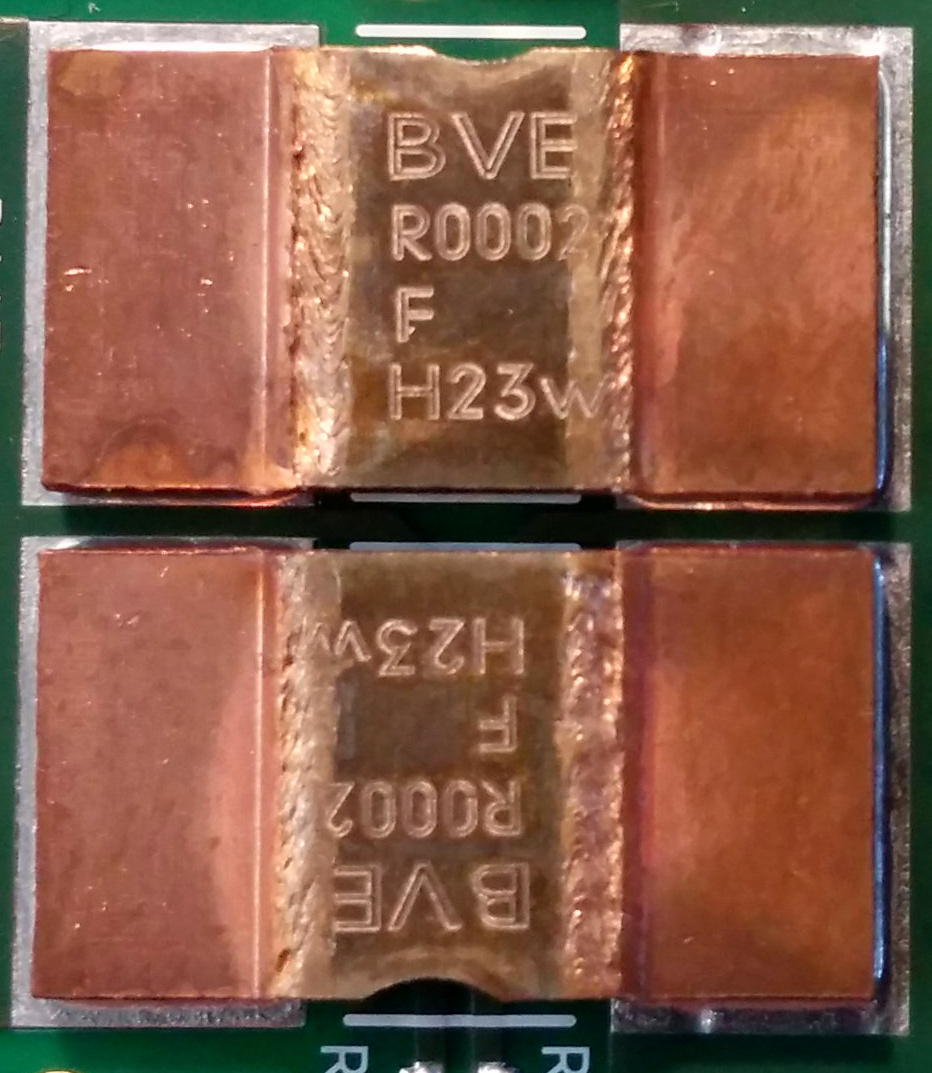
\includegraphics[height=1.15cm]{../figures/d5_smd_shunt.jpg}\hspace{2mm}%
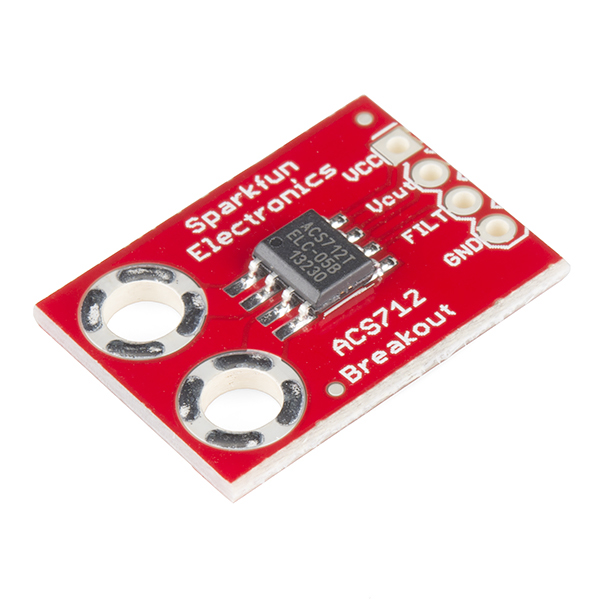
\includegraphics[height=1.15cm]{../figures/d5_hall_current.jpg}\\
\credit{SMD shunts: wdwd, CC BY-SA 4.0; Hall IC: SparkFun, CC BY 2.0; via Wikimedia Commons}
\column{.55\textwidth}
\scriptsize
\renewcommand{\arraystretch}{1.15}
\begin{tabularx}{\linewidth}{@{}l X X X@{}}
\toprule
 & \textbf{Shunt} & \textbf{Hall OL\,/\,CL} & \textbf{Fluxgate}\\
\midrule
Isolation & no (needs isol.\ amp / $\Sigma\Delta$) & yes & yes\\
Accuracy & 0.1--0.5\,\% & 1--3\,\% / 0.2--0.5\,\% & $<$0.1\,\%\\
Offset drift & very low & medium & very low\\
Bandwidth & DC--MHz & DC--\SIrange{50}{300}{kHz} & DC--\SIrange{10}{200}{kHz}\\
Losses & $I^2R$ & small & small\\
Cost / size & lowest & medium & highest\\
\bottomrule
\end{tabularx}

\vspace{1mm}
\begin{itemize}\scriptsize
\item Hall: $u_H\propto B\propto i$ in a slotted core; closed loop nulls the flux with a compensation winding.
\item Fluxgate: a periodically saturated core detects zero flux $\Rightarrow$ very low offset.
\item Offset in $i_a,i_b$ gives a torque ripple at $f_\text{el}$; gain mismatch at $2f_\text{el}$.
\end{itemize}
\end{columns}
\end{frame}

% ---------------------------------------------------------------------
\begin{frame}{Force: strain gauges and load cells}
\begin{columns}[T]
\column{.36\textwidth}
\centering
\begin{circuitikz}[scale=.5,transform shape,font=\scriptsize]
  \draw (0,0) node[left]{} to[R,l=$R_1$] (2,2) to[R,l=$R_2$] (4,0);
  \draw (0,0) to[R,l_=$R_4$] (2,-2) to[R,l_=$R_3$] (4,0);
  \draw (0,0) -- (0,-2.8) to[V,l_=$U_\text{ex}$] (4,-2.8) -- (4,0);
  \draw (2,2) to[short,*-o] (2,2.5) node[above]{$u_+$};
  \draw (2,-2) to[short,*-o] (2,-1.5) node[right]{$u_-$};
\end{circuitikz}

\vspace{1mm}
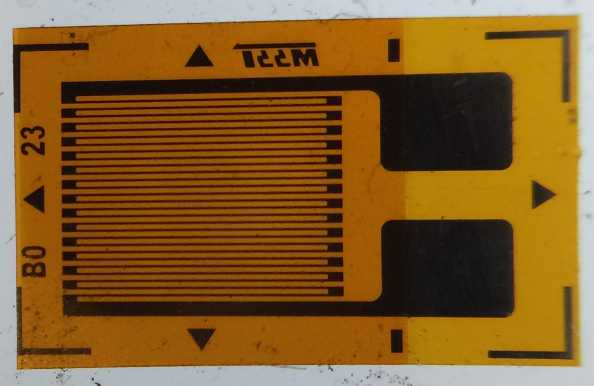
\includegraphics[height=1.7cm]{../figures/d5_strain_gauge.jpg}\hspace{1mm}%
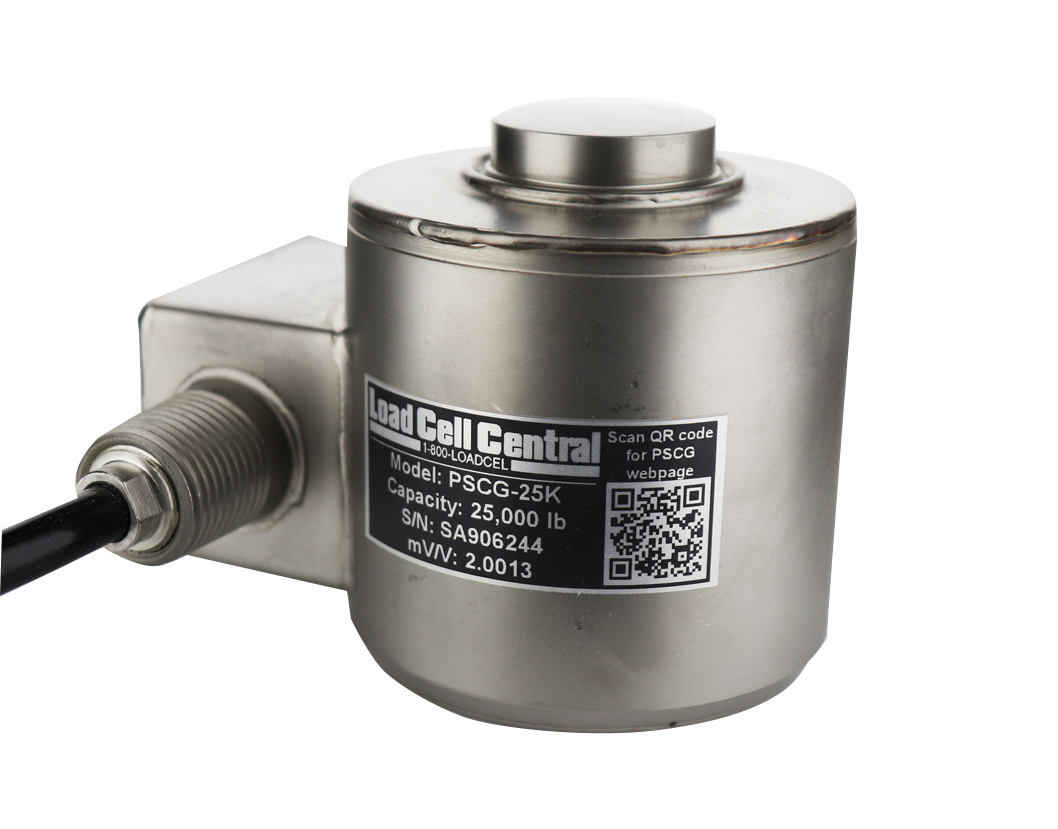
\includegraphics[height=1.7cm]{../figures/d5_load_cell.jpg}\\
\credit{Foil gauge: Pleriche, CC BY-SA 4.0; load cell: Daraceleste, CC BY-SA 4.0; via Wikimedia Commons}
\column{.62\textwidth}
\begin{eqbox}
\vspace{-2mm}
\[
\frac{\Delta R}{R}=k_\text{GF}\,\varepsilon,\qquad
\frac{u_\text{out}}{U_\text{ex}}\approx\frac{k_\text{GF}\,\varepsilon}{4}\,n_\text{active}
\]
\vspace{-4mm}
\end{eqbox}
\begin{itemize}\footnotesize
\item Metal foil gauge: gauge factor $k_\text{GF}\approx 2$; strains are $\mu$-level.
\item \term{Full bridge} (4 active arms, $\pm\varepsilon$): 4$\times$ sensitivity, temperature compensation, rejects bending.
\item Example: $\varepsilon=\SI{1000}{\micro\epsilon}$, $U_\text{ex}=\SI{5}{V}$, full bridge: $u_\text{out}=2\cdot10^{-3}\cdot\SI{5}{V}=\SI{10}{mV}$.
\item Load cells are specified by rated output, e.g.\ \SI{2}{mV/V} at nominal force $\Rightarrow$ need a low-noise instrumentation amplifier or 24-bit $\Sigma\Delta$ ADC.
\item Errors: creep, hysteresis, temperature of zero and span, non-linearity ($\sim$0.02--0.1\,\% FS).
\end{itemize}
\end{columns}
\end{frame}

% ---------------------------------------------------------------------
\begin{frame}{Temperature: NTC, PT100/PT1000, thermocouple, KTY}
\begin{columns}[T]
\column{.5\textwidth}
\centering
\begin{tikzpicture}
\begin{axis}[mkplot,width=\linewidth,height=4.3cm,ymode=log,xmin=-40,xmax=200,ymin=100,ymax=4e5,
  xlabel={temperature $\vartheta$ [\si{\celsius}]},ylabel={resistance [\si{\ohm}]},legend pos=north east]
\addplot[mkBlue,thick] table[x=T,y=pt]{\dat{temp}};
\addplot[mkOrange,thick] table[x=T,y=ntc]{\dat{temp}};
\legend{PT1000 (IEC 60751), NTC \SI{10}{k\ohm}, $B=3950$}
\end{axis}
\end{tikzpicture}\\[1mm]
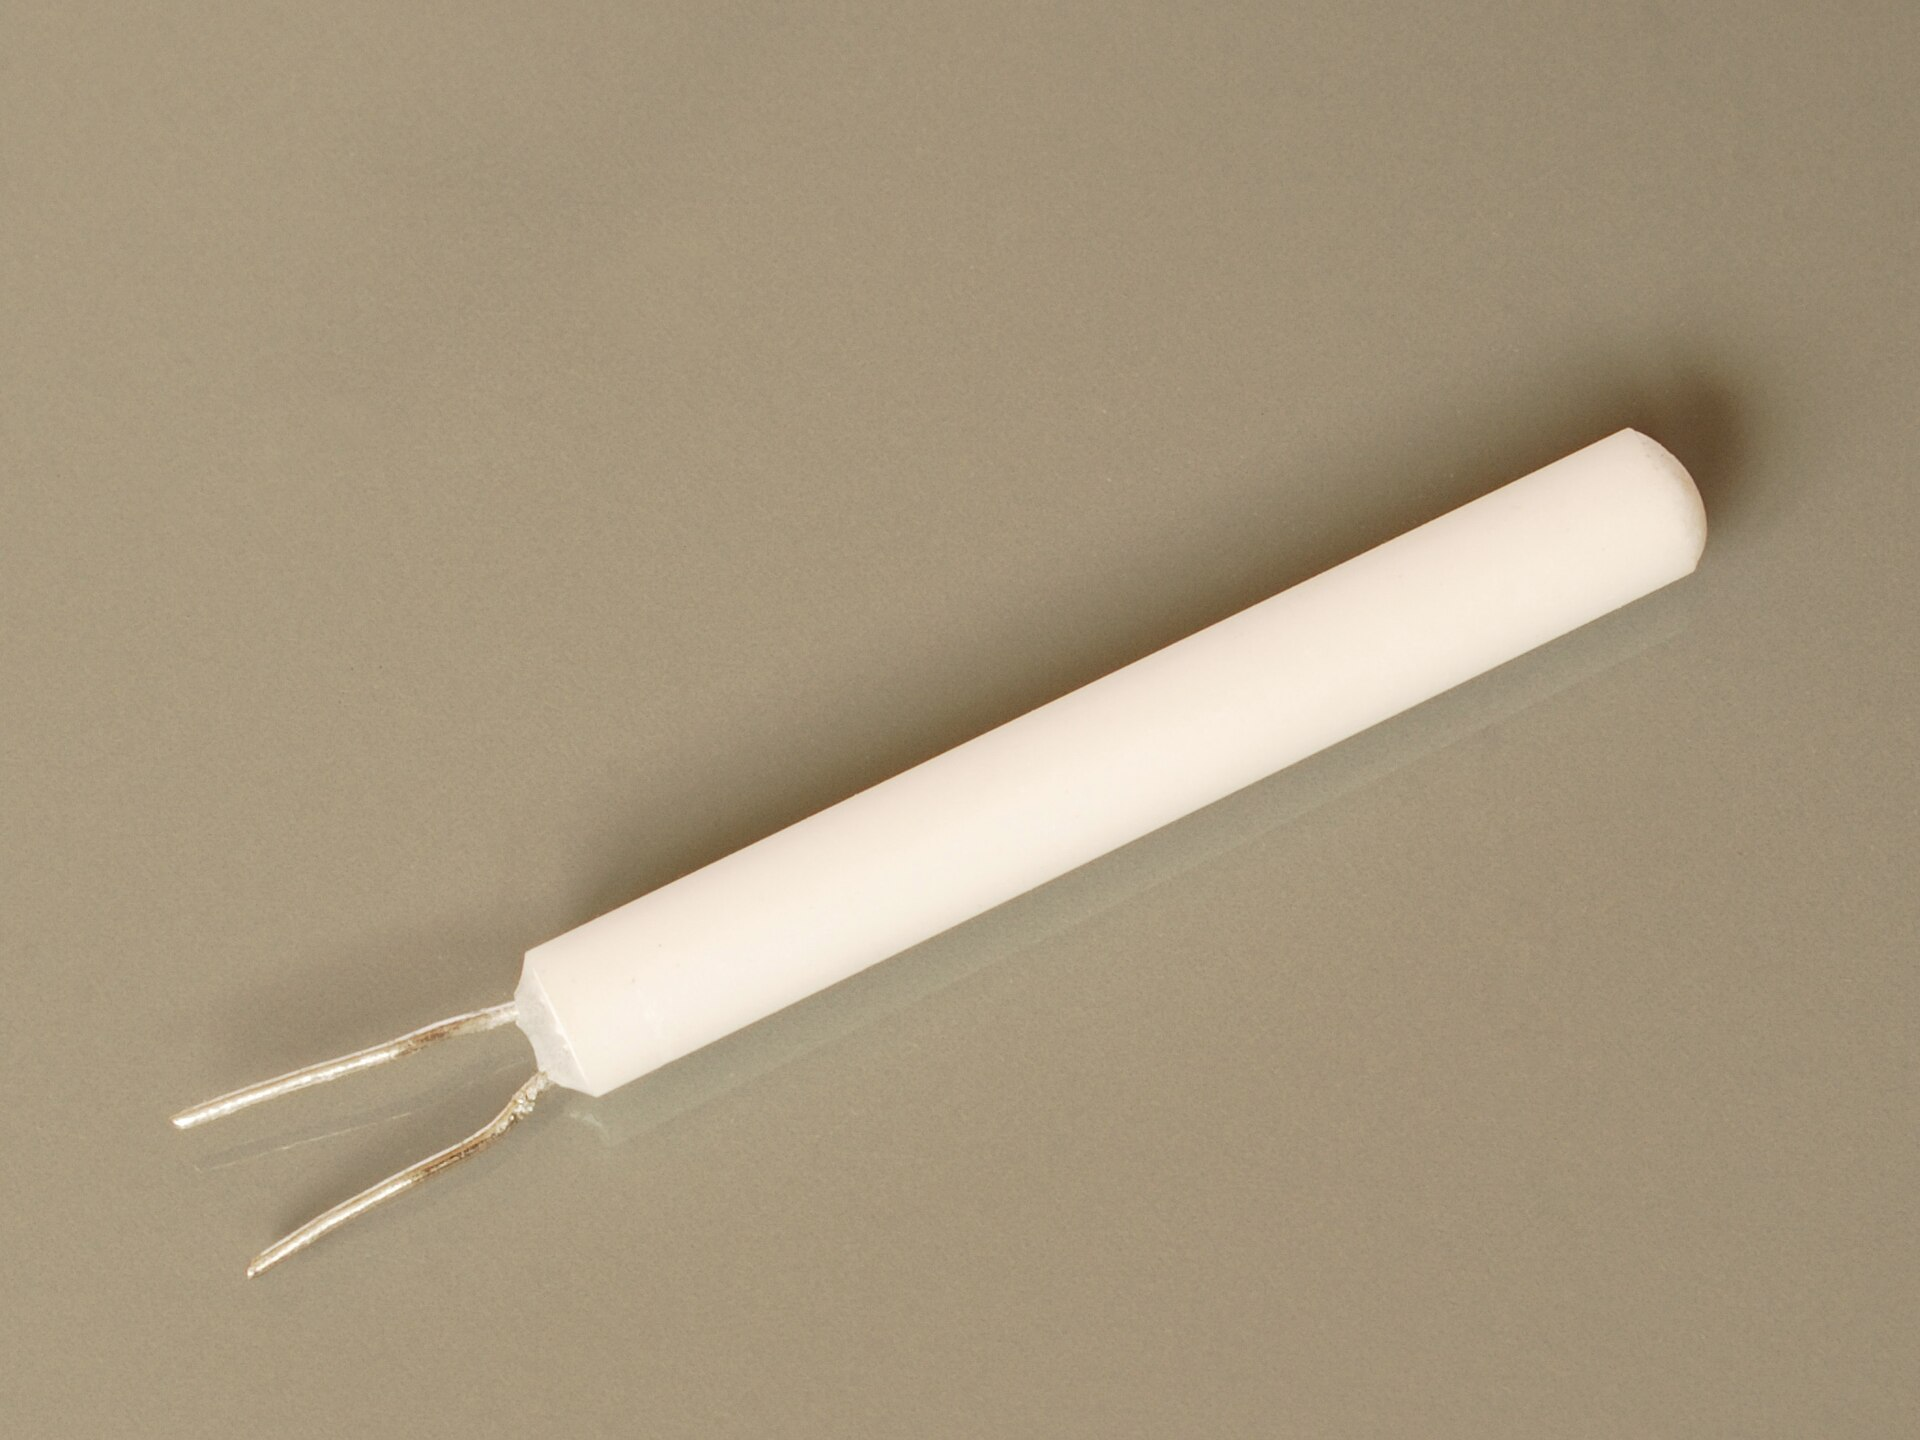
\includegraphics[height=1.75cm]{../figures/d5_pt100.jpg}\hspace{2mm}%
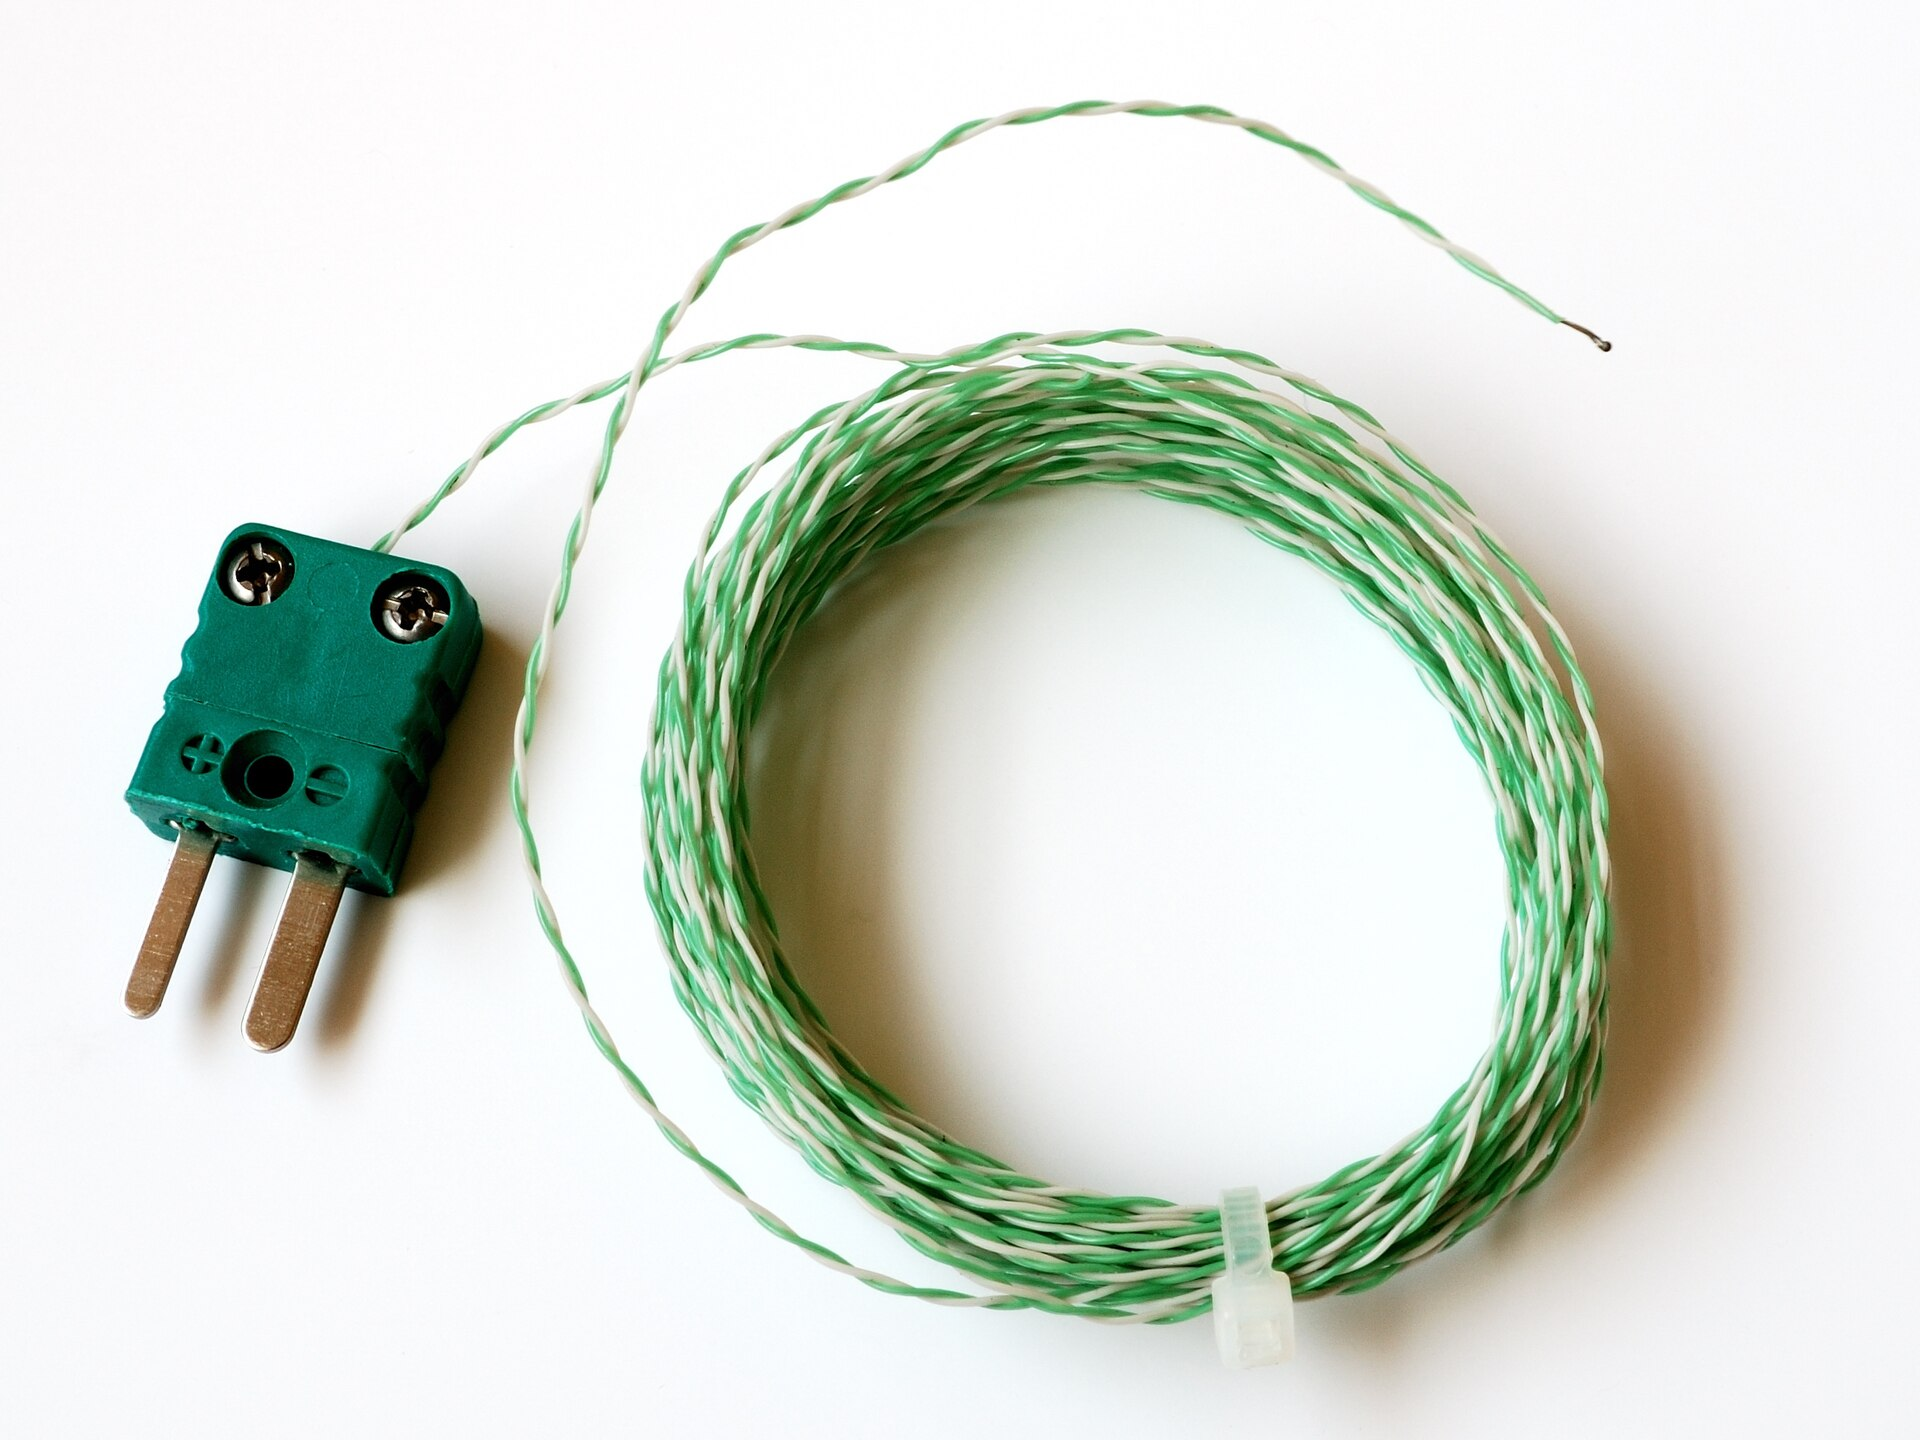
\includegraphics[height=1.75cm]{../figures/d5_thermocouple.jpg}\\
\credit{Left: wire-wound Pt100, Harke, CC BY-SA 3.0; right: type-K thermocouple, Harke, public domain; both via Wikimedia Commons}
\column{.48\textwidth}
\footnotesize
\textbf{PT100/PT1000} ($\vartheta\ge\SI{0}{\celsius}$, Callendar--Van Dusen):
\[ R=R_0(1+A\vartheta+B\vartheta^2) \]\vspace{-4mm}\[\scriptstyle A=3.9083\cdot10^{-3}\,\mathrm{K}^{-1},\ B=-5.775\cdot10^{-7}\,\mathrm{K}^{-2}\]
\textbf{NTC}: $R=R_{25}\exp\!\big[B\,(1/T-1/T_{25})\big]$, $T$ in K.
\begin{itemize}\scriptsize
\item \term{PT}: linear, accurate (class A: $\pm(0.15+0.002|\vartheta|)$\,K), 3/4-wire.
\item \term{NTC}: very sensitive, non-linear; IGBT modules, heatsinks.
\item \term{Thermocouple}: Seebeck voltage, type K $\approx\SI{41}{\micro V/K}$, needs cold-junction compensation.
\item \term{KTY} (silicon PTC, e.g.\ KTY84: \SI{1}{k\ohm} at \SI{100}{\celsius}): motor winding, used for thermal models; PTC triplets for trip only.
\end{itemize}
\end{columns}
\end{frame}

% ---------------------------------------------------------------------
\begin{frame}{Summary: sensors and measurement principles}
\begin{columns}[T]
\column{.55\textwidth}
\begin{itemize}\small
\item Specify sensors with the full vocabulary: accuracy, precision, resolution, range, repeatability, linearity.
\item Currents: shunt (cheap, accurate, needs isolation), Hall (isolated, drift), fluxgate (precision).
\item Force: strain-gauge bridges deliver mV/V --- amplifier noise and drift dominate.
\item Temperature: PT for accuracy, NTC for sensitivity, thermocouple for high $\vartheta$, KTY in motors.
\end{itemize}
\column{.42\textwidth}
\begin{keybox}[Checklist for any sensor]
\footnotesize
\checkitem\ What error matters: offset, gain, noise or drift?\\
\checkitem\ Bandwidth and latency vs.\ loop $f_c$\\
\checkitem\ Isolation and EMC environment\\
\checkitem\ Calibration and diagnostics
\end{keybox}
{\scriptsize\color{mkGray} [Fraden, 2016]; IEC 60751; manufacturer notes (TI, ADI, LEM-type sensor datasheets).}
\end{columns}
\end{frame}

% =====================================================================
\section{Encoder and resolver (4.2)}

\begin{frame}{Optical incremental encoders}
\begin{columns}[T]
\column{.45\textwidth}
\centering
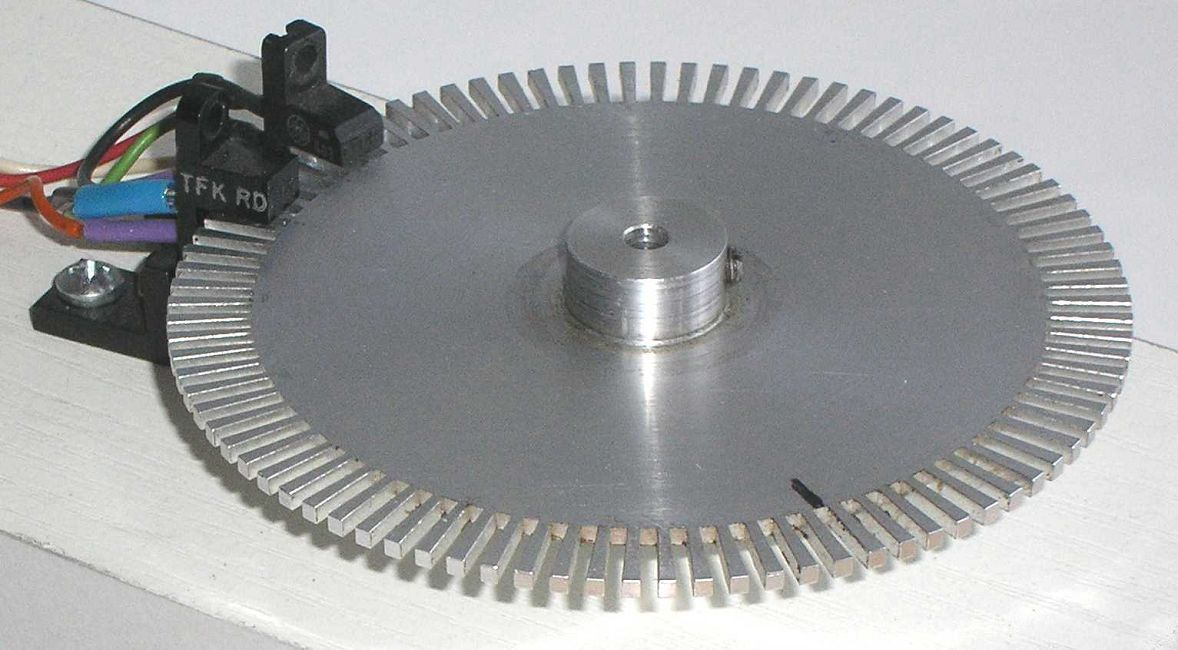
\includegraphics[width=\linewidth,height=4.2cm,keepaspectratio]{../figures/d5_encoder_model.jpg}\\
\credit{Rrudzik, CC BY-SA 4.0, via Wikimedia Commons}
\column{.52\textwidth}
\begin{itemize}\footnotesize
\item LED $\to$ code disk with $N$ lines (PPR) $\to$ phase-shifted gratings $\to$ photodiodes.
\item Outputs: \term{A}, \term{B} (\SI{90}{\degree} shifted) and \term{Z} (index, once per rev.), usually RS-422 differential.
\item Edge counting gives position relative to power-up $\Rightarrow$ \hl{homing} needed.
\item Max.\ output frequency $f_\text{A}=N\,n/60$; e.g.\ $N=2500$, $n=\SI{6000}{rpm}$ $\Rightarrow$ \SI{250}{kHz} (\SI{1}{MHz} edge rate).
\item Also magnetic (Hall / MR) and inductive variants: robust, lower resolution.
\end{itemize}
\end{columns}
\end{frame}

% ---------------------------------------------------------------------
\begin{frame}{Quadrature signals and $\times4$ decoding}
\begin{columns}[T]
\column{.62\textwidth}
\centering
\begin{tikzpicture}[xscale=.62,yscale=.62,font=\scriptsize]
  % A
  \node[left] at (0,4.4) {A};
  \draw[mkBlue,thick] (0,4) -- (1,4) -- (1,5) -- (3,5) -- (3,4) -- (5,4) -- (5,5) -- (7,5) -- (7,4) -- (9,4) -- (9,5) -- (11,5) -- (11,4) -- (12,4);
  % B
  \node[left] at (0,2.4) {B};
  \draw[mkOrange,thick] (0,2) -- (2,2) -- (2,3) -- (4,3) -- (4,2) -- (6,2) -- (6,3) -- (8,3) -- (8,2) -- (10,2) -- (10,3) -- (12,3);
  % Z
  \node[left] at (0,0.4) {Z};
  \draw[mkMid,thick] (0,0) -- (5,0) -- (5,1) -- (6,1) -- (6,0) -- (12,0);
  % edges
  \foreach \x in {1,2,3,4,5,6,7,8,9,10,11}{ \draw[mkGray,dotted] (\x,-0.3) -- (\x,5.3); }
  \foreach \x/\c in {1/1,2/2,3/3,4/4,5/5,6/6,7/7,8/8,9/9,10/10,11/11}{ \node[font=\tiny,mkGray] at (\x,-0.6) {\c}; }
  \draw[{Latex}-{Latex},mkNavy] (1,5.6) -- (5,5.6) node[midway,above]{1 line = $360^\circ_\text{el}$};
  \draw[{Latex}-{Latex},mkOrange] (1,3.5) -- (2,3.5) node[midway,above,font=\tiny]{$90^\circ$};
  \node[mkGray,font=\tiny,anchor=west] at (12.1,-0.6) {count};
\end{tikzpicture}
\column{.36\textwidth}
\scriptsize
\renewcommand{\arraystretch}{1.05}
\begin{tabular}{@{}c c c@{}}
\toprule
prev.\ AB & new AB & count\\
\midrule
00 & 10 & $+1$\\
10 & 11 & $+1$\\
11 & 01 & $+1$\\
01 & 00 & $+1$\\
\multicolumn{2}{c}{reverse order} & $-1$\\
\multicolumn{2}{c}{both change} & error\\
\bottomrule
\end{tabular}

\vspace{1mm}
\begin{itemize}\scriptsize
\item Every edge of A and B is counted: $4N$ counts/rev.
\item Direction from which channel leads (A leads $\Rightarrow$ forward).
\item Both bits changing at once = lost count $\Rightarrow$ error flag.
\item Digital glitch filter limits max.\ edge rate.
\end{itemize}
\end{columns}
\end{frame}

% ---------------------------------------------------------------------
\begin{frame}{Absolute encoders, Gray code and serial protocols}
\begin{columns}[T]
\column{.3\textwidth}
\centering
\begin{tikzpicture}[scale=.75]
  % 3-bit Gray code disk: rings bit2 (inner) .. bit0 (outer)
  \foreach \k/\b/\c/\d in {0/0/0/0,1/0/0/1,2/0/1/1,3/0/1/0,4/1/1/0,5/1/1/1,6/1/0/1,7/1/0/0}{
    \pgfmathsetmacro{\aa}{90-\k*45}\pgfmathsetmacro{\ab}{90-(\k+1)*45}
    \ifnum\b=1 \fill[mkBlue] (\aa:.35) arc (\aa:\ab:.35) -- (\ab:.6) arc (\ab:\aa:.6) -- cycle; \fi
    \ifnum\c=1 \fill[mkMid] (\aa:.6) arc (\aa:\ab:.6) -- (\ab:.85) arc (\ab:\aa:.85) -- cycle; \fi
    \ifnum\d=1 \fill[mkOrange] (\aa:.85) arc (\aa:\ab:.85) -- (\ab:1.1) arc (\ab:\aa:1.1) -- cycle; \fi
    \draw[mkGray,very thin] (\aa:.35) -- (\aa:1.1);
    \pgfmathsetmacro{\am}{90-\k*45-22.5}
    \node[font=\tiny,mkNavy] at (\am:1.3) {\b\c\d};
  }
  \draw[mkGray] (0,0) circle (.35) circle (.6) circle (.85) circle (1.1);
\end{tikzpicture}
\\{\scriptsize 3-bit Gray-code disk}\\[1mm]
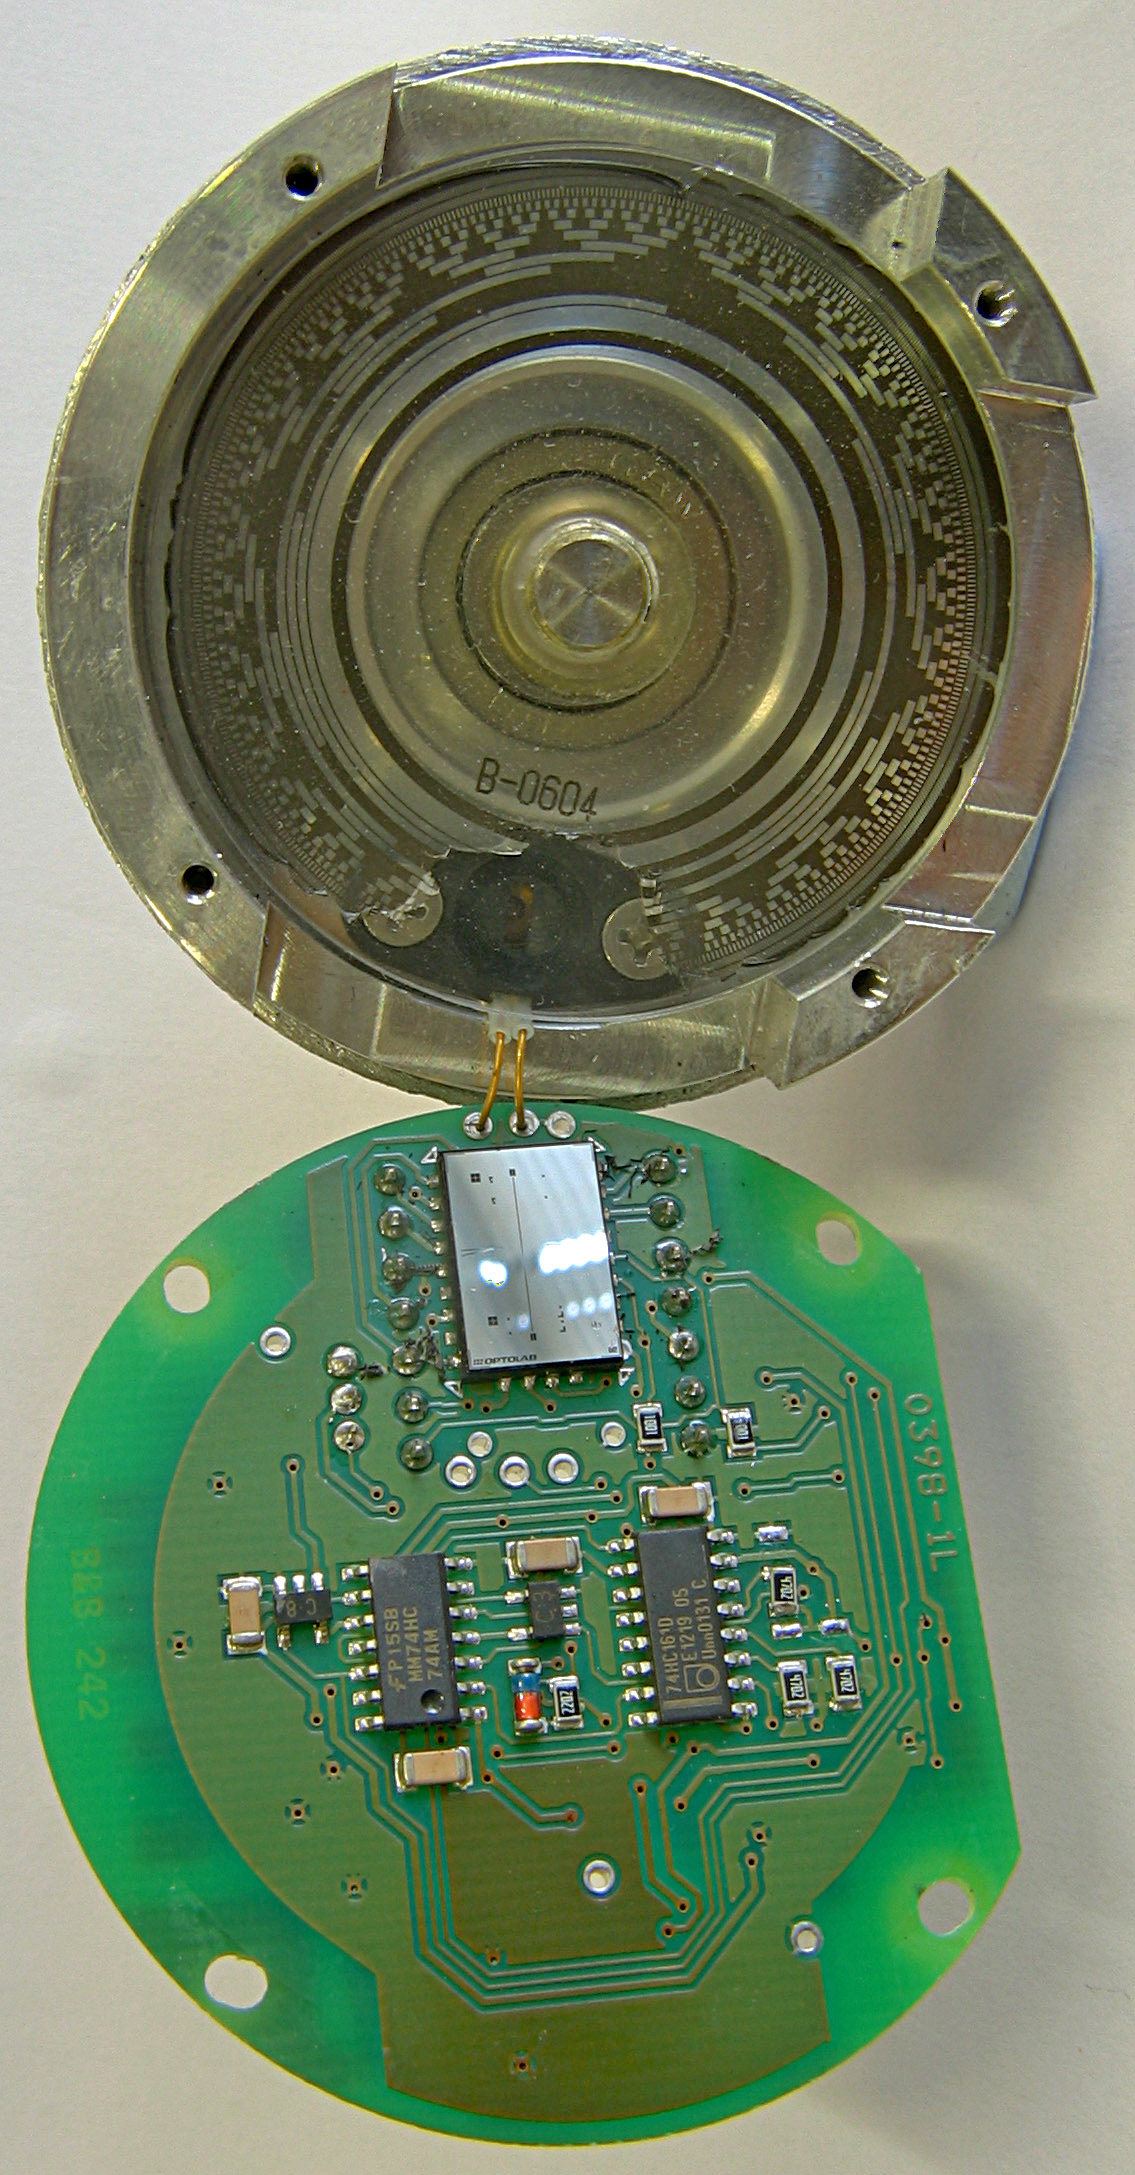
\includegraphics[height=2.3cm]{../figures/d5_gray_encoder.jpg}\\
\credit{13-track Gray-code encoder, Mike1024, public domain, via Wikimedia Commons}
\column{.68\textwidth}
\begin{itemize}\footnotesize
\item \term{Single-turn}: unique code per angle, e.g.\ 23 bit $=8\,388\,608$ positions/rev. \term{Multi-turn}: + 12--16 bit revolution counter (gear stages, battery or Wiegand energy harvesting).
\item \term{Gray code}: only one bit changes per step $\Rightarrow$ no false codes at transitions; $g=b\oplus(b\gg1)$.
\end{itemize}
\scriptsize
\renewcommand{\arraystretch}{1.08}
\begin{tabularx}{\linewidth}{@{}l l X@{}}
\toprule
\textbf{Protocol} & \textbf{Physical} & \textbf{Features}\\
\midrule
SSI & RS-422, clock + data & unidirectional, simple, no CRC by default, $\sim$\SI{1}{MHz}\\
BiSS-C & RS-422 & open, bidirectional registers, CRC, line-delay comp., up to \SI{10}{MHz}\\
EnDat 2.2 & RS-485 & bidirectional, CRC, diagnostics, electronic ID label, up to \SI{16}{MHz}\\
One-cable (DSL) & RS-485 in motor cable & digital link via power cable, saves connector\\
\bottomrule
\end{tabularx}
\end{columns}
\end{frame}

% ---------------------------------------------------------------------
\begin{frame}{Sin/cos encoders and interpolation}
\begin{columns}[T]
\column{.4\textwidth}
\centering
\begin{tikzpicture}
\begin{axis}[mkplot,width=5.4cm,height=5.4cm,axis equal image,xmin=-1.4,xmax=1.4,ymin=-1.4,ymax=1.4,
  xlabel={$u_\text{cos}$},ylabel={$u_\text{sin}$},legend style={at={(0.5,1.02)},anchor=south},legend columns=2]
\addplot[mkBlue,thick,domain=0:360,samples=100] ({cos(x)},{sin(x)});
\addplot[mkOrange,thick,domain=0:360,samples=100] ({0.15+1.1*cos(x)},{0.9*sin(x+12)});
\legend{ideal, offset+gain+phase err.}
\draw[mkNavy,-{Latex}] (axis cs:0,0) -- (axis cs:{cos(50)},{sin(50)}) node[above right,font=\tiny]{$\phi$};
\end{axis}
\end{tikzpicture}
\column{.58\textwidth}
\begin{itemize}\footnotesize
\item Analogue tracks: $u_\text{sin}=\hat U\sin(N\theta)$, $u_\text{cos}=\hat U\cos(N\theta)$, typ.\ \SI{1}{V_{pp}}, $N=512$--$2048$ periods/rev.
\item Coarse position: count periods; fine position inside one period:
\end{itemize}
\begin{eqbox}
\vspace{-2mm}
\[
\theta = \frac{2\pi}{N}\left(m + \frac{\operatorname{atan2}(u_\text{sin},u_\text{cos})}{2\pi}\right)
\]
\vspace{-4mm}
\end{eqbox}
\begin{itemize}\footnotesize
\item $N=2048$ with 12-bit interpolation $\Rightarrow 2^{23}$ counts/rev.
\item Error harmonics per signal period: \hl{offset $\to$ 1st}, \hl{amplitude mismatch, phase error $\to$ 2nd}; corrected by online calibration of the Lissajous ellipse.
\item Interpolation accuracy is limited by signal quality, noise and ADC resolution, not by the arithmetic.
\end{itemize}
\end{columns}
\end{frame}

% ---------------------------------------------------------------------
\begin{frame}{Resolver: principle and signals}
\begin{columns}[T]
\column{.55\textwidth}
\centering
\begin{tikzpicture}
\begin{groupplot}[group style={group size=1 by 3,vertical sep=1.5mm,xticklabels at=edge bottom},
  mkplot,width=\linewidth,xmin=0,xmax=10,ymin=-1.1,ymax=1.1,ytick=\empty]
\nextgroupplot[height=2.2cm,ylabel={$u_\text{ex}$}]
\addplot[mkMid,thin] table[x=t,y=e]{\dat{resolver}};
\nextgroupplot[height=2.2cm,ylabel={$u_\text{sin}$},ymin=-.6,ymax=.6]
\addplot[mkBlue,thin] table[x=t,y=s]{\dat{resolver}};
\addplot[mkOrange,thick,dashed] table[x=t,y=es]{\dat{resolver}};
\nextgroupplot[height=2.2cm,ylabel={$u_\text{cos}$},ymin=-.6,ymax=.6,xlabel={time [ms]}]
\addplot[mkBlue,thin] table[x=t,y=c]{\dat{resolver}};
\addplot[mkOrange,thick,dashed] table[x=t,y=ec]{\dat{resolver}};
\end{groupplot}
\end{tikzpicture}
{\scriptsize\color{mkGray} Illustration: carrier \SI{2}{kHz} (real: \SIrange{5}{20}{kHz}), $\theta$ ramping at 100 rev/s.}
\column{.43\textwidth}
\begin{minipage}[t]{.36\linewidth}\vspace{0pt}
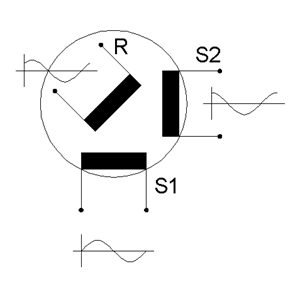
\includegraphics[width=\linewidth]{../figures/d5_resolver_principle.png}\\
\credit{Hasee, public domain, via Wikimedia Commons}
\end{minipage}\hfill
\begin{minipage}[t]{.6\linewidth}\vspace{0pt}
\begin{itemize}\footnotesize
\item Rotary transformer: rotor winding R excited by $u_\text{ex}=\hat U\sin\omega_e t$.
\item Two stator windings S1, S2 \SI{90}{\degree} apart:
\end{itemize}
\end{minipage}
\vspace{-2mm}
\begin{align*}
u_\text{sin}&=k_r\hat U\sin(\omega_e t)\,\sin(p_r\theta)\\
u_\text{cos}&=k_r\hat U\sin(\omega_e t)\,\cos(p_r\theta)
\end{align*}
\vspace{-5mm}
\begin{itemize}\footnotesize
\item Angle is in the \hl{envelopes} (dashed); $k_r\approx0.5$, $p_r$ = speed (pole-pair) count.
\item No electronics in the motor: robust to \SI{150}{\celsius}+, shock, vibration; typ.\ accuracy \SIrange{5}{10}{arcmin}.
\end{itemize}
\end{columns}
\end{frame}

% ---------------------------------------------------------------------
\begin{frame}{Resolver-to-digital conversion: the tracking loop}
\centering
\begin{tikzpicture}[font=\scriptsize,node distance=7mm]
  \node[blk] (m1) {$\times\cos\hat\phi$};
  \node[blk,below=4mm of m1] (m2) {$\times\sin\hat\phi$};
  \node[sumn,right=9mm of $(m1)!.5!(m2)$] (sub) {};
  \node[blk,right=of sub] (dem) {synchronous\\demodulator};
  \node[blk,right=of dem] (pi) {PI\\$K_p+K_i/s$};
  \node[blk,right=of pi] (int) {$\dfrac{1}{s}$};
  \coordinate[right=12mm of int] (o);
  \draw[sig] ($(m1.west)+(-1.3,0)$) -- (m1) node[pos=0,left]{$u_\text{sin}$};
  \draw[sig] ($(m2.west)+(-1.3,0)$) -- (m2) node[pos=0,left]{$u_\text{cos}$};
  \draw[sig] (m1.east) -| (sub) node[pos=.9,left]{$+$};
  \draw[sig] (m2.east) -| (sub) node[pos=.9,left]{$-$};
  \draw[sig] (sub) -- (dem); \draw[sig] (dem) -- (pi) node[midway,above]{$\varepsilon$};
  \draw[sig] (pi) -- (int) node[midway,above]{$\hat\omega$};
  \draw[sig] (int) -- (o) node[right]{$\hat\phi$};
  \draw[sig] ($(int.east)+(5mm,0)$) -- ++(0,-1.7) -| ($(m2.south)+(-.3,0)$) node[pos=.3,below]{sin/cos of $\hat\phi$ (LUT)};
  \draw[sig] ($(pi.east)+(3mm,0)$) -- ++(0,.9) node[above]{velocity output};
  \node[lbl] at ($(dem)+(0,.75)$) {ref.\ $u_\text{ex}$};
\end{tikzpicture}

\vspace{2mm}
\begin{columns}[T]
\column{.5\textwidth}
\begin{eqbox}
\vspace{-2mm}
\[
\varepsilon\propto \sin p_r\theta\cos\hat\phi-\cos p_r\theta\sin\hat\phi=\sin(p_r\theta-\hat\phi)
\]
\vspace{-4mm}
\end{eqbox}
\begin{itemize}\footnotesize
\item For small errors $\varepsilon\approx p_r\theta-\hat\phi$: a \term{type-II} PLL.
\end{itemize}
\column{.47\textwidth}
\begin{itemize}\footnotesize
\item Zero steady-state error at constant speed; acceleration error $\propto \alpha/K_a$.
\item Loop bandwidth (typ.\ \SIrange{1}{5}{kHz}) trades noise vs.\ lag.
\item Integrated RDC ICs (e.g.\ AD2S1210-class) or software RDC in the drive MCU / FPGA.
\end{itemize}
\end{columns}
\end{frame}

% ---------------------------------------------------------------------
\begin{frame}{Velocity from position: M-, T- and M/T-method}
\begin{columns}[T]
\column{.5\textwidth}
\centering
\begin{tikzpicture}[xscale=.55,yscale=.55,font=\tiny]
  % pulses
  \foreach \x in {0.7,2.3,3.9,5.5,7.1,8.7,10.3}{ \draw[mkBlue,thick] (\x,0) -- (\x,1) -- (\x+.8,1) -- (\x+.8,0);}
  \draw[mkBlue,thick] (0,0) -- (11.5,0);
  \node[left] at (0,.5) {edges};
  % sample instants
  \foreach \x in {1.5,9.5}{ \draw[mkOrange,thick,dashed] (\x,-2.6) -- (\x,1.6);}
  \draw[{Latex}-{Latex},mkOrange] (1.5,1.9) -- (9.5,1.9) node[midway,above]{$T_s$ (M: count $m_1$ edges)};
  % T method
  \draw[{Latex}-{Latex},mkMid] (2.3,-1.0) -- (3.9,-1.0) node[midway,below]{T: $m$ clocks};
  % MT window
  \draw[{Latex}-{Latex},mkNavy] (2.3,-2.2) -- (10.3,-2.2) node[midway,below]{M/T: $T_\text{det}$ (edge to edge)};
  \draw[mkNavy,dotted] (2.3,-2.4) -- (2.3,0); \draw[mkNavy,dotted] (10.3,-2.4) -- (10.3,0);
\end{tikzpicture}

\vspace{2mm}
\scriptsize
\renewcommand{\arraystretch}{1.1}
\begin{tabularx}{\linewidth}{@{}l X X@{}}
\toprule
 & \textbf{good at} & \textbf{weak at}\\
\midrule
M & high speed & low speed (few counts)\\
T & low speed & high speed (few clocks), no edge $\Rightarrow$ no update\\
M/T & whole range & needs edge time-stamping HW\\
\bottomrule
\end{tabularx}
\column{.48\textwidth}
With $4N$ counts/rev, clock $f_\text{clk}$:
\begin{eqbox}
\footnotesize
\vspace{-2mm}
\begin{align*}
\text{M:}\quad &\omega=\frac{2\pi\,m_1}{4N\,T_s}\\
\text{T:}\quad &\omega=\frac{2\pi}{4N}\cdot\frac{f_\text{clk}}{m}\\
\text{M/T:}\quad &\omega=\frac{2\pi\,m_1}{4N}\cdot\frac{f_\text{clk}}{m_2}
\end{align*}
\vspace{-5mm}
\end{eqbox}
\begin{itemize}\footnotesize
\item M/T: count $m_1$ edges and $m_2$ clocks over a window that starts and ends on an edge (window $\ge T_s$).
\item Modern drives: \term{edge time-stamping} + absolute high-resolution position.
\end{itemize}
\end{columns}
\end{frame}

% ---------------------------------------------------------------------
\begin{frame}{Low-speed limits and quantisation noise}
\begin{columns}[T]
\column{.52\textwidth}
\centering
\begin{tikzpicture}
\begin{axis}[mkplot,width=\linewidth,height=5.3cm,xmode=log,ymode=log,xmin=0.1,xmax=6000,ymin=1e-4,ymax=1e3,
  xlabel={speed $n$ [rpm]},ylabel={relative quantisation error [\%]},legend pos=north west]
\addplot[mkBlue,thick] table[x=n,y=M]{\dat{velmeas}};
\addplot[mkOrange,thick] table[x=n,y=T]{\dat{velmeas}};
\addplot[mkSky,thick,dashed] table[x=n,y=MT]{\dat{velmeas}};
\legend{M-method, T-method, M/T}
\end{axis}
\end{tikzpicture}
{\scriptsize\color{mkGray} $N=2500$ lines, $T_s=\SI{125}{\micro s}$, $f_\text{clk}=\SI{100}{MHz}$.}
\column{.46\textwidth}
\begin{keybox}[Worked example]
\footnotesize\raggedright
M-method resolution: $\Delta n=\dfrac{60}{4N\,T_s}=\dfrac{60}{10^4\cdot125\cdot10^{-6}}=\SI{48}{rpm}$.\\[1mm]
At \SI{60}{rpm} the raw estimate jumps between 48 and \SI{96}{rpm}!\\[1mm]
Differencing uniform position noise ($\sigma_\theta=q/\sqrt{12}$):
\[
\sigma_\omega=\frac{\sqrt2\,q}{\sqrt{12}\,T_s}=0.41\,\frac{q}{T_s}\approx\SI{20}{rpm}
\]
23-bit absolute encoder: $\Delta n=\SI{0.057}{rpm}$.
\end{keybox}
\begin{itemize}\scriptsize
\item Remedies: higher resolution, longer window, edge timing, observer or filter (next sessions).
\end{itemize}
\end{columns}
\end{frame}

% ---------------------------------------------------------------------
\begin{frame}{Summary: encoder and resolver}
\begin{columns}[T]
\column{.55\textwidth}
\begin{itemize}\small
\item Incremental A/B/Z: $\times4$ decoding, homing required, simple and fast.
\item Absolute single/multi-turn: Gray code internally, serial protocols (SSI, BiSS-C, EnDat) with CRC.
\item Sin/cos: interpolation by atan2; offset/gain/phase errors produce 1st/2nd harmonics.
\item Resolver: robust analogue sensor; RDC = type-II tracking loop.
\item Velocity estimation is a \hl{quantisation} problem at low speed.
\end{itemize}
\column{.42\textwidth}
\scriptsize
\renewcommand{\arraystretch}{1.12}
\begin{tabular}{@{}l c c c@{}}
\toprule
 & \textbf{incr.} & \textbf{abs.} & \textbf{resolver}\\
\midrule
Resolution & med. & \textcolor{mkGreen}{high} & med.\\
Absolute & \textcolor{mkRed}{no} & \textcolor{mkGreen}{yes} & 1 turn\\
Robustness & med. & med. & \textcolor{mkGreen}{high}\\
Diagnostics & low & \textcolor{mkGreen}{high} & med.\\
Cost & \textcolor{mkGreen}{low} & high & med.\\
\bottomrule
\end{tabular}

\vspace{2mm}
{\scriptsize\color{mkGray} [Krishnan, 2010]; ADI and TI resolver / encoder application notes; EnDat, BiSS and SSI interface specifications.}
\end{columns}
\end{frame}

% =====================================================================
\section{Sampling and digitisation (4.3)}

\begin{frame}{ADC architectures for drives: SAR and sigma-delta}
\begin{columns}[T]
\column{.5\textwidth}
\centering
\resizebox{\linewidth}{!}{\begin{tikzpicture}[font=\scriptsize,node distance=5mm]
  \node[blk] (sh) {S/H};
  \node[blk,right=of sh] (cmp) {comp.};
  \node[blk,right=of cmp] (sar) {SAR\\logic};
  \node[blk,below=4mm of cmp] (dac) {DAC};
  \draw[sig] ($(sh.west)+(-.6,0)$) -- (sh) node[pos=0,left]{$u$};
  \draw[sig] (sh) -- (cmp); \draw[sig] (cmp) -- (sar);
  \draw[sig] (sar.south) |- (dac); \draw[sig] (dac) -| ($(cmp.south)+(-.15,0)$);
  \draw[sig] (sar.east) -- ++(.5,0) node[right]{$N$ bit};
  \node[lbl,above=1mm of cmp] {SAR: binary search, $N$ steps};
\end{tikzpicture}}

\vspace{3mm}
\resizebox{\linewidth}{!}{\begin{tikzpicture}[font=\scriptsize,node distance=5mm]
  \node[sumn] (s) {};
  \node[blk,right=of s] (in) {$\int$};
  \node[blk,right=of in] (q) {1-bit\\quant.};
  \node[blk,right=8mm of q,fill=mkCream,draw=mkOrange] (dec) {sinc$^3$\\decimation};
  \draw[sig] ($(s.west)+(-.5,0)$) -- (s) node[pos=0,left]{$u$};
  \draw[sig] (s) -- (in); \draw[sig] (in) -- (q); \draw[sig] (q) -- (dec) node[midway,above]{bit stream};
  \draw[sig] (dec.east) -- ++(.4,0) node[right]{$N$ bit};
  \draw[sig] ($(q.east)+(2mm,0)$) -- ++(0,-.7) -| (s) node[pos=.95,left]{$-$};
  \node[lbl,above=1mm of in] {$\Sigma\Delta$: oversampling + noise shaping};
\end{tikzpicture}}
\column{.48\textwidth}
\scriptsize
\renewcommand{\arraystretch}{1.12}
\begin{tabularx}{\linewidth}{@{}l X X@{}}
\toprule
 & \textbf{SAR} & \textbf{Sigma-delta}\\
\midrule
Resolution & 12--16 bit & 16--24 bit\\
Rate & 1--5 MS/s & kS/s--MS/s (after decim.)\\
Latency & \textcolor{mkGreen}{1 conversion} & \textcolor{mkRed}{filter group delay}\\
Sampling instant & sharp (S/H) & averaged over window\\
Typical use & phase currents, on-chip MCU ADC & isolated current meas., load cells, temperatures\\
\bottomrule
\end{tabularx}

\vspace{1mm}
\begin{notebox}
Isolated $\Sigma\Delta$ modulators next to the shunt + sinc filter in MCU/FPGA are standard for high-performance current measurement.
\end{notebox}
\end{columns}
\end{frame}

% ---------------------------------------------------------------------
\begin{frame}{Quantisation and $\text{SNR}=6.02N+1.76$ dB}
\begin{columns}[T]
\column{.5\textwidth}
\centering
\begin{tikzpicture}
\begin{groupplot}[group style={group size=1 by 2,vertical sep=2mm,xticklabels at=edge bottom},
  mkplot,width=\linewidth,xmin=0,xmax=1]
\nextgroupplot[height=3.6cm,ymin=-1.1,ymax=1.1,ylabel={signal},legend pos=north east]
\addplot[mkSky,thick] table[x=t,y=x]{\dat{quant}};
\addplot[mkBlue,thick,const plot] table[x=t,y=xq]{\dat{quant}};
\legend{$x$, 3-bit $x_q$}
\nextgroupplot[height=2.4cm,ymin=-.6,ymax=.6,ylabel={$e/q$},xlabel={time (one period)}]
\addplot[mkOrange,thin] table[x=t,y=e]{\dat{quant}};
\end{groupplot}
\end{tikzpicture}
\column{.48\textwidth}
\footnotesize
Step $q=2U_\text{FS}/2^N$; error uniform in $[-q/2,q/2]$:
\[
P_e=\frac{q^2}{12},\qquad P_s=\frac{1}{2}\Big(\frac{2^N q}{2}\Big)^2=\frac{2^{2N}q^2}{8}
\]
\begin{eqbox}
\vspace{-2mm}
\[
\begin{aligned}\text{SNR}&=10\log_{10}\tfrac{P_s}{P_e}=10\log_{10}\!\big(1.5\cdot 2^{2N}\big)\\&=6.02N+1.76\ \text{dB}\end{aligned}
\]
\vspace{-4mm}
\end{eqbox}
\begin{itemize}\scriptsize
\item 12 bit: \SI{74}{dB}; 16 bit: \SI{98}{dB} (full-scale sine).
\item Real ADCs: $\text{ENOB}=(\text{SINAD}-1.76)/6.02$, often 1--2 bit below $N$.
\item Example: $\pm\SI{50}{A}$ range, 12 bit $\Rightarrow$ LSB $=\SI{24.4}{mA}$.
\item Oversampling by $M$ + averaging: $+10\log_{10}M$ dB if noise is white.
\end{itemize}
\end{columns}
\end{frame}

% ---------------------------------------------------------------------
\begin{frame}{Aliasing and the Nyquist criterion}
\begin{columns}[T]
\column{.58\textwidth}
\centering
\begin{tikzpicture}
\begin{axis}[mkplot,width=\linewidth,height=4.6cm,xmin=0,xmax=20,ymin=-1.3,ymax=1.5,
  xlabel={time [ms]},ylabel={amplitude},legend pos=north east,legend columns=3]
\addplot[mkSky,thin] table[x=t,y=x]{\dat{alias_c}};
\addplot[mkOrange,thick,dashed] table[x=t,y=a]{\dat{alias_c}};
\addplot[mkBlue,only marks,mark=*,mark size=1.4pt] table[x=t,y=x]{\dat{alias_s}};
\legend{\SI{900}{Hz} signal, \SI{100}{Hz} alias, samples $f_s=\SI{1}{kHz}$}
\end{axis}
\end{tikzpicture}

\begin{tikzpicture}[xscale=1.0,font=\tiny]
  \draw[-{Latex},mkGray] (0,0) -- (8.2,0) node[right]{$f$};
  \foreach \x/\l in {0/0,2/{$f_s/2$},4/{$f_s$},6/{$3f_s/2$},8/{$2f_s$}}{\draw (\x,0) -- (\x,-.1) node[below]{\l};}
  \draw[mkGreen,thick] (0,0) -- (0,.05);
  \fill[mkPale,opacity=.6] (0,0) rectangle (2,.9); \node[mkNavy] at (1.5,1.05) {base band};
  \draw[mkBlue,very thick,-{Latex}] (3.6,0) -- (3.6,.7) node[above]{\SI{900}{Hz}};
  \draw[mkOrange,very thick,-{Latex}] (0.4,0) -- (0.4,.7) node[above]{\SI{100}{Hz}};
  \draw[mkOrange,-{Latex},dashed,bend right=30] (3.6,.35) to (0.4,.35);
\end{tikzpicture}
\column{.4\textwidth}
\begin{eqbox}
\vspace{-2mm}
\[
f_\text{alias}=\left|f-k\,f_s\right|,\quad k=\operatorname{round}(f/f_s)
\]
\vspace{-4mm}
\end{eqbox}
\begin{itemize}\footnotesize
\item Nyquist: a signal is uniquely represented only if $f_\text{max}<f_s/2$.
\item Content above $f_s/2$ \hl{folds} into the base band and is indistinguishable from real low-frequency signals.
\item Classical drive example: PWM ripple, encoder interpolation errors or a resonance aliasing onto the velocity loop.
\item Once sampled, aliasing \emph{cannot} be removed by any digital filter.
\end{itemize}
\end{columns}
\end{frame}

% ---------------------------------------------------------------------
\begin{frame}{Synchronous sampling with PWM, timestamps and latency}
\begin{columns}[T]
\column{.55\textwidth}
\centering
\begin{tikzpicture}[font=\scriptsize,xscale=.95]
  % carrier
  \draw[mkGray,thin] (0,0) -- (6.4,0);
  \draw[mkMid,thick] (0,0) -- (1.6,1.6) -- (3.2,0) -- (4.8,1.6) -- (6.4,0);
  \draw[mkOrange,thick] (0,.9) -- (6.4,.9) node[right]{$d$};
  \node[mkMid,left] at (0,1.2) {carrier};
  % gate
  \draw[mkBlue,thick] (0,-.6) -- (.9,-.6) -- (.9,-.2) -- (2.3,-.2) -- (2.3,-.6) -- (4.1,-.6) -- (4.1,-.2) -- (5.5,-.2) -- (5.5,-.6) -- (6.4,-.6);
  \node[mkBlue,left] at (0,-.4) {$s_a$};
  % current ripple
  \draw[mkNavy,thick] (0,-1.6) -- (.9,-1.9) -- (2.3,-1.3) -- (4.1,-1.9) -- (5.5,-1.3) -- (6.4,-1.6);
  \draw[mkGray,dashed] (0,-1.6) -- (6.4,-1.6);
  \node[mkNavy,left] at (0,-1.6) {$i_a$};
  % sample points
  \foreach \x/\y in {0/-1.6,3.2/-1.6,6.4/-1.6,1.6/-1.6,4.8/-1.6}{\fill[mkOrange] (\x,\y) circle (.07);}
  \foreach \x in {0,3.2,6.4}{\draw[mkOrange,dashed] (\x,-2.1) -- (\x,0);}
  \node[mkOrange,below,align=center] at (3.2,-2.1) {sample at carrier valley/peak\\$=$ mean of ripple, far from edges};
\end{tikzpicture}

\vspace{2mm}
\begin{tikzpicture}[font=\tiny,xscale=.95]
  \draw[thick,fill=mkPale] (0,0) rectangle (.6,.4) node[midway]{S/H};
  \draw[thick,fill=mkPale] (.6,0) rectangle (1.5,.4) node[midway]{ADC};
  \draw[thick,fill=mkCream] (1.5,0) rectangle (3.6,.4) node[midway]{FOC computation};
  \draw[thick,fill=mkPale] (3.6,0) rectangle (6.4,.4) node[midway]{new duty active};
  \draw[{Latex}-{Latex}] (0,-.15) -- (3.2,-.15) node[midway,below]{$T_s$};
  \draw[{Latex}-{Latex},mkOrange] (0,.6) -- (4.8,.6) node[midway,above]{effective delay $T_d\approx1.5\,T_s$};
\end{tikzpicture}
\column{.43\textwidth}
\begin{itemize}\footnotesize
\item Centre-aligned PWM: sampling at the carrier peak/valley returns the \hl{average} current without ripple or switching noise $\Rightarrow$ no extra filter.
\item Single or double update ($f_s=f_\text{PWM}$ or $2f_\text{PWM}$).
\item Time-stamp every sample (encoder, current, bus) on a common time base.
\end{itemize}
\begin{keybox}[Delay $\to$ phase]
\footnotesize
$f_s=\SI{16}{kHz}$, $T_d=1.5T_s=\SI{94}{\micro s}$: phase lag at \SI{1}{kHz}
$\ 360^\circ\cdot f\,T_d=34^\circ$ --- comparable to the whole PM budget of the current loop.
\end{keybox}
\end{columns}
\end{frame}



% ---------------------------------------------------------------------
\begin{frame}{Summary: sampling and digitisation}
\begin{columns}[T]
\column{.55\textwidth}
\begin{itemize}\small
\item SAR for low latency, $\Sigma\Delta$ for resolution and isolation.
\item Ideal quantisation: $\text{SNR}=6.02N+1.76$ dB; check ENOB in practice.
\item Anything above $f_s/2$ folds back: filter \emph{before} sampling.
\item Sample synchronously with PWM; time-stamp all measurements.
\item Every sample of delay is phase lag: $360^\circ f T_d$.
\end{itemize}
\column{.42\textwidth}
\begin{keybox}[Remember]
\footnotesize
Resolution, noise, bandwidth and delay of the measurement chain set the achievable loop bandwidth --- not the controller structure.
\end{keybox}
{\scriptsize\color{mkGray} [Oppenheim \& Schafer, 2010]; [Franklin, Powell \& Workman, 1998]; ADI/TI ADC application notes.}
\end{columns}
\end{frame}
% =====================================================================
\section{Signal processing and filters (4.4)}

\begin{frame}{Filter types at a glance}
\centering
\begin{tikzpicture}
\begin{groupplot}[group style={group size=4 by 1,horizontal sep=6mm,yticklabels at=edge left},
  mkplot,width=4.2cm,height=3.6cm,xmode=log,xmin=0.05,xmax=20,ymin=-40,ymax=5,
  xlabel={$\omega/\omega_0$},xtick={0.1,1,10},xticklabels={0.1,1,10}]
\nextgroupplot[title={\scriptsize Low-pass},ylabel={$|H|$ [dB]}]
\addplot[mkBlue,thick,domain=0.05:20,samples=150]{-10*log10(1+x^4)};
\addplot[mkSky,dashed,domain=0.05:20,samples=150]{-10*log10(1+x^2)};
\nextgroupplot[title={\scriptsize High-pass}]
\addplot[mkBlue,thick,domain=0.05:20,samples=150]{-10*log10(1+x^(-4))};
\addplot[mkSky,dashed,domain=0.05:20,samples=150]{-10*log10(1+x^(-2))};
\nextgroupplot[title={\scriptsize Band-pass ($Q=2$)}]
\addplot[mkOrange,thick,domain=0.05:20,samples=300]{-10*log10(1+4*(x-1/x)^2)};
\nextgroupplot[title={\scriptsize Band-stop / notch}]
\addplot[mkOrange,thick,domain=0.05:20,samples=400]{10*log10(max((1-x^2)^2,1e-5)/((1-x^2)^2+(x)^2))};
\end{groupplot}
\end{tikzpicture}

\vspace{2mm}
\scriptsize
\renewcommand{\arraystretch}{1.12}
\begin{tabularx}{\linewidth}{@{}l l X@{}}
\toprule
\textbf{Type} & \textbf{2nd-order prototype} & \textbf{Typical use in a drive}\\
\midrule
LPF & $\omega_0^2/(s^2+2\zeta\omega_0 s+\omega_0^2)$ & noise on velocity / torque reference, anti-aliasing\\
HPF & $s^2/(s^2+2\zeta\omega_0 s+\omega_0^2)$ & remove offset / drift (AC coupling), wash-out in feed-forward\\
BPF & $2\zeta\omega_0 s/(s^2+2\zeta\omega_0 s+\omega_0^2)$ & extract a known frequency (vibration monitoring, resolver carrier)\\
BSF & $(s^2+\omega_0^2)/(s^2+2\zeta\omega_0 s+\omega_0^2)$ & resonance suppression, mains / ripple rejection\\
\bottomrule
\end{tabularx}
\end{frame}

% ---------------------------------------------------------------------
\begin{frame}{First-order low-pass: from $H(s)$ to a difference equation}
\begin{columns}[T]
\column{.5\textwidth}
\[
H(s)=\frac{\omega_f}{s+\omega_f}
\]
\begin{itemize}\footnotesize
\item \term{Exact (ZOH / impulse-invariant)}:
\end{itemize}
\begin{eqbox}
\vspace{-2mm}
\[
y[k]=y[k-1]+\alpha\,\big(x[k]-y[k-1]\big)
\]
\vspace{-6mm}
\[
\alpha=1-e^{-\omega_f T_s}
\]
\vspace{-4mm}
\end{eqbox}
\begin{itemize}\footnotesize
\item \term{Tustin}: $s\to\frac{2}{T_s}\frac{z-1}{z+1}$, matches the frequency response better near $f_s/2$.
\item First-order HPF: $y_\text{HP}[k]=x[k]-y_\text{LP}[k]$ (complementary pair).
\item Small $\omega_f T_s$: $\alpha\approx\omega_f T_s$ (\hl{exponential smoothing}).
\end{itemize}
\column{.47\textwidth}
\begin{keybox}[Worked example]
\footnotesize
$f_f=\SI{500}{Hz}$, $f_s=\SI{16}{kHz}$ ($T_s=\SI{62.5}{\micro s}$):
\[
\omega_fT_s=2\pi\cdot500\cdot62.5\cdot10^{-6}=0.196
\]
\[
\alpha=1-e^{-0.196}=0.178
\]
Group delay at low $f$: $1/\omega_f=\SI{318}{\micro s}\approx 5$ samples.
\end{keybox}
\begin{notebox}
Every low-pass filter in a loop is a delay of roughly $1/\omega_f$ at low frequency: include it in the loop model.
\end{notebox}
\end{columns}
\end{frame}

% ---------------------------------------------------------------------
\begin{frame}{Moving average: a simple FIR filter}
\begin{columns}[T]
\column{.55\textwidth}
\centering
\begin{tikzpicture}
\begin{axis}[mkplot,width=\linewidth,height=5.3cm,xmin=0,xmax=0.5,ymin=-40,ymax=3,
  xlabel={normalised frequency $f/f_s$},ylabel={$|H|$ [dB]},legend pos=north east]
\addplot[mkBlue,thick] table[x=f,y=N4]{\dat{mavg}};
\addplot[mkOrange,thick] table[x=f,y=N8]{\dat{mavg}};
\addplot[mkSky,thick] table[x=f,y=N16]{\dat{mavg}};
\legend{$N=4$,$N=8$,$N=16$}
\end{axis}
\end{tikzpicture}
\column{.43\textwidth}
\begin{eqbox}
\vspace{-2mm}
\[
y[k]=\frac1N\sum_{i=0}^{N-1}x[k-i]
\]
\[
|H(e^{j\Omega})|=\left|\frac{\sin(N\Omega/2)}{N\sin(\Omega/2)}\right|
\]
\vspace{-4mm}
\end{eqbox}
\begin{itemize}\footnotesize
\item \term{Sinc-like} magnitude, zeros at $f=k\,f_s/N$: cancels a known periodic disturbance exactly (choose $N T_s$ = its period).
\item Linear phase, group delay $\frac{N-1}{2}T_s$.
\item Poor stop-band (first side lobe only \SI{-13}{dB}).
\item Recursive form: $y[k]=y[k-1]+\frac{x[k]-x[k-N]}{N}$.
\end{itemize}
\end{columns}
\end{frame}

% ---------------------------------------------------------------------
\begin{frame}{FIR versus IIR filters}
\begin{columns}[T]
\column{.5\textwidth}
\centering
\begin{tikzpicture}[font=\scriptsize,node distance=4mm]
  \node (x) at (0,0) {$x[k]$};
  \node[blk,minimum width=7mm] (d1) at (1.5,0) {$z^{-1}$};
  \node[blk,minimum width=7mm] (d2) at (3.0,0) {$z^{-1}$};
  \node at (4.0,0) {$\cdots$};
  \foreach \i/\xx in {0/0.6,1/2.25,2/3.75}{
    \node[draw=mkOrange,thick,isosceles triangle,shape border rotate=-90,inner sep=1pt,font=\tiny] (b\i) at (\xx,-.9) {$b_\i$};
    \draw[sig] (\xx,0) -- (b\i);
  }
  \draw[sig] (x) -- (d1); \draw[sig] (d1) -- (d2);
  \node[sumn] (sm) at (4.6,-1.8) {+};
  \foreach \i in {0,1,2}{ \draw[sig] (b\i) |- (sm); }
  \draw[sig] (sm) -- ++(.8,0) node[right]{$y[k]$};
  \node[lbl,anchor=west] at (-.3,.55) {FIR: only feed-forward taps};
\end{tikzpicture}

\vspace{4mm}
\begin{tikzpicture}[font=\scriptsize]
  \node (x) at (0,0) {$x[k]$};
  \node[sumn] (s) at (1.2,0) {+};
  \node[blk] (b) at (2.5,0) {$b_0$};
  \draw[sig] (x) -- (s); \draw[sig] (s) -- (b); \draw[sig] (b) -- ++(1.2,0) node[right]{$y[k]$};
  \node[blk,minimum width=7mm] (d) at (3.0,-1.0) {$z^{-1}$};
  \node[draw=mkOrange,thick,isosceles triangle,shape border rotate=180,inner sep=1pt,font=\tiny] (a) at (1.9,-1.0) {$-a_1$};
  \draw[sig] (3.4,0) |- (d); \draw[sig] (d) -- (a); \draw[sig] (a) -| (s);
  \node[lbl,anchor=west] at (-.3,.55) {IIR: output fed back};
\end{tikzpicture}
\column{.48\textwidth}
\scriptsize
\renewcommand{\arraystretch}{1.15}
\begin{tabularx}{\linewidth}{@{}l X X@{}}
\toprule
 & \textbf{FIR} & \textbf{IIR}\\
\midrule
Structure & taps only & taps + feedback\\
Stability & \textcolor{mkGreen}{always} & \textcolor{mkRed}{poles inside unit circle}\\
Phase & \textcolor{mkGreen}{linear possible} (symmetric $b_i$) & non-linear\\
Order needed & \textcolor{mkRed}{high} (tens--hundreds) & \textcolor{mkGreen}{low} (2--8)\\
Cost / sample & $N$ MAC & $\sim$5 MAC per biquad\\
Delay & $(N{-}1)T_s/2$ & small, $f$-dependent\\
Quantisation & robust & use biquads\\
\bottomrule
\end{tabularx}

\vspace{1mm}
{\footnotesize In loops \hl{IIR} wins (low delay); FIR for linear phase.}
\end{columns}
\end{frame}

% ---------------------------------------------------------------------
\begin{frame}{Butterworth vs.\ Bessel: magnitude, group delay, step response}
\begin{columns}[T]
\column{.5\textwidth}
\centering
\begin{tikzpicture}
\begin{groupplot}[group style={group size=1 by 2,vertical sep=3mm,xticklabels at=edge bottom},
  mkplot,width=\linewidth,xmode=log,xmin=50,xmax=10000]
\nextgroupplot[height=3.5cm,ymin=-60,ymax=5,ylabel={$|H|$ [dB]},legend pos=south west]
\addplot[mkBlue,thick] table[x=f,y=mb]{\dat{bwbs}};
\addplot[mkOrange,thick] table[x=f,y=ms]{\dat{bwbs}};
\legend{Butterworth 4th, Bessel 4th}
\nextgroupplot[height=3.0cm,ymin=0,ymax=0.7,ylabel={$\tau_g$ [ms]},xlabel={$f$ [Hz], $f_c=\SI{1}{kHz}$ (\SI{-3}{dB})}]
\addplot[mkBlue,thick] table[x=f,y=gb]{\dat{bwbs}};
\addplot[mkOrange,thick] table[x=f,y=gs]{\dat{bwbs}};
\end{groupplot}
\end{tikzpicture}
\column{.48\textwidth}
\centering
\begin{tikzpicture}
\begin{axis}[mkplot,width=\linewidth,height=3.6cm,xmin=0,xmax=3,ymin=0,ymax=1.2,
  xlabel={time [ms]},ylabel={step response},legend pos=south east]
\addplot[mkBlue,thick] table[x=t,y=b]{\dat{bwbs_step}};
\addplot[mkOrange,thick] table[x=t,y=s]{\dat{bwbs_step}};
\addplot[mkGray,thin,dashed,domain=0:3,samples=2]{1};
\legend{overshoot 10.8\,\%, overshoot 0.8\,\%}
\end{axis}
\end{tikzpicture}
\begin{itemize}\scriptsize
\item \term{Butterworth}: $|H|^2=1/(1+(\omega/\omega_c)^{2n})$, maximally flat magnitude; \SI{-38}{dB} at $3f_c$; $\tau_g$ peaks near $f_c$ $\Rightarrow$ ringing.
\item \term{Bessel}: maximally flat group delay $\tau_g=-\mathrm{d}\varphi/\mathrm{d}\omega$, near-linear phase, clean step; only \SI{-25}{dB} at $3f_c$.
\item Butterworth for attenuation (AAF, noise), Bessel for waveform fidelity (transients).
\end{itemize}
\end{columns}
\end{frame}

% ---------------------------------------------------------------------
\begin{frame}{Filtered derivative: position $\to$ velocity $\to$ acceleration}
\begin{columns}[T]
\column{.48\textwidth}
\centering
\begin{tikzpicture}
\begin{axis}[mkplot,width=\linewidth,height=5.0cm,xmode=log,xmin=1,xmax=10000,ymin=0,ymax=80,
  xlabel={frequency $f$ [Hz]},ylabel={$|D(j\omega)|$ [dB re 1/s]},legend pos=north west]
\addplot[mkSky,thick,dashed,domain=1:10000,samples=100]{20*log10(2*pi*x)};
\addplot[mkBlue,thick,domain=1:10000,samples=200]{20*log10(2*pi*x/sqrt(1+(x/300)^2))};
\addplot[mkOrange,thick,domain=1:10000,samples=200]{20*log10(2*pi*x/(1+(x/300)^2))};
\legend{ideal $s$, $s/(1+sT_f)$, $s/(1+sT_f)^2$}
\end{axis}
\end{tikzpicture}
{\scriptsize\color{mkGray} $f_f=1/(2\pi T_f)=\SI{300}{Hz}$.}
\column{.5\textwidth}
\begin{itemize}\footnotesize
\item Differentiation \hl{amplifies} high frequencies by $\omega$ (+\SI{20}{dB/dec}); quantisation noise is broad-band.
\item Practical derivative: $D(s)=\dfrac{s}{1+sT_f}$, high-frequency gain limited to $1/T_f$.
\end{itemize}
\begin{eqbox}
\footnotesize
\vspace{-2mm}
\[
\sigma_\omega=\frac{\sqrt2}{T_s}\,\frac{q}{\sqrt{12}},\qquad
\sigma_\alpha=\frac{\sqrt6}{T_s^2}\,\frac{q}{\sqrt{12}}
\]
\vspace{-4mm}
\end{eqbox}
\begin{itemize}\footnotesize
\item (Backward differences; coefficient energy $1^2{+}1^2$ and $1^2{+}2^2{+}1^2$.)
\item $q=2\pi/10^4$, $T_s=\SI{125}{\micro s}$: $\sigma_\alpha\approx\SI{2.8e4}{rad/s^2}$ --- useless unfiltered.
\item Better: \term{observer} / tracking loop (model-based, Day 3) instead of raw differences.
\end{itemize}
\end{columns}
\end{frame}

% ---------------------------------------------------------------------
\begin{frame}{Velocity from a quantised encoder: raw vs.\ filtered}
\begin{columns}[T]
\column{.62\textwidth}
\centering
\begin{tikzpicture}
\begin{axis}[mkplot,width=\linewidth,height=5.6cm,xmin=0,xmax=50,ymin=-10,ymax=160,
  xlabel={time [ms]},ylabel={speed [rpm]},legend pos=north east,legend columns=3]
\addplot[mkSky,thin] table[x=t,y=r]{\dat{velnoise}};
\addplot[mkOrange,thick] table[x=t,y=f]{\dat{velnoise}};
\addplot[mkNavy,thick,dashed] table[x=t,y=w]{\dat{velnoise}};
\legend{raw difference, 2nd-order LPF \SI{150}{Hz}, true}
\end{axis}
\end{tikzpicture}
\column{.36\textwidth}
\footnotesize
Simulation: $N=2500$ lines ($\times4$), $T_s=\SI{125}{\micro s}$, true speed $60\pm\SI{30}{rpm}$ at \SI{20}{Hz}.
\begin{itemize}\footnotesize
\item Raw $\Delta\theta/T_s$ takes only values $0,48,96,\dots$ rpm.
\item The LPF recovers the trend but adds \hl{phase lag} ($\approx$\SI{1.5}{ms} at low $f$) and residual ripple.
\item Loop gain multiplies this noise into the torque command $\Rightarrow$ audible noise, heating.
\item Root cause is \emph{resolution}, filtering is only a compromise.
\end{itemize}
\end{columns}
\end{frame}

% ---------------------------------------------------------------------
\begin{frame}{Anti-aliasing: analogue before the ADC, digital after}
\begin{columns}[T]
\column{.55\textwidth}
\centering
\begin{tikzpicture}[font=\scriptsize]
  \draw[-{Latex},mkGray] (0,0) -- (7,0) node[right]{$f$};
  \draw[-{Latex},mkGray] (0,0) -- (0,2.4) node[above]{$|X|$};
  \draw[mkGray,dashed] (3,0) -- (3,2.2) node[above]{$f_s/2$};
  \draw[mkGray,dashed] (6,0) -- (6,2.2) node[above]{$f_s$};
  % signal band
  \fill[mkPale] (0,0) rectangle (1.4,1.6); \node at (.7,1.8) {signal};
  % noise
  \draw[mkRed,thick] (4.2,0) -- (4.2,1.2) node[above]{noise};
  \draw[mkRed,-{Latex},dashed] (4.2,.6) to[bend left=35] (1.8,.6);
  \node[mkRed] at (2.4,.15) {alias};
  % AAF
  \draw[mkOrange,very thick] (0,2.0) -- (1.8,2.0) .. controls (2.6,2.0) and (2.9,.3) .. (4.5,.1) -- (6.8,.05);
  \node[mkOrange,anchor=west] at (4.6,1.9) {analogue AAF};
\end{tikzpicture}

\vspace{2mm}
\begin{tikzpicture}[font=\scriptsize,node distance=5mm]
  \node[blk] (s) {sensor};
  \node[blk,right=of s,fill=mkCream,draw=mkOrange] (aaf) {analogue\\RC / 2nd order};
  \node[blk,right=of aaf] (adc) {ADC\\$f_s$ (high)};
  \node[blk,right=of adc] (dig) {digital LPF\\+ decimate};
  \draw[sig] (s) -- (aaf); \draw[sig] (aaf) -- (adc); \draw[sig] (adc) -- (dig);
  \draw[sig] (dig) -- ++(1,0) node[right]{$f_s/M$};
\end{tikzpicture}
\column{.43\textwidth}
\begin{itemize}\footnotesize
\item Only an \hl{analogue} filter in front of the sampler prevents aliasing.
\item Oversampling ($f_s\gg$ signal band) relaxes the analogue filter to a simple RC; the sharp filter is then done digitally before decimation.
\item $\Sigma\Delta$ converters are the extreme case: very high modulator rate, sinc decimation.
\item In a control loop, the analogue AAF adds delay too --- keep its corner $\ge 5$--$10\times f_c$ and include it in the model.
\item Synchronous sampling of PWM ripple (previous session) is a ``structural'' anti-aliasing measure.
\end{itemize}
\end{columns}
\end{frame}

% ---------------------------------------------------------------------
\begin{frame}[fragile]{Implementing filters: difference equations and biquads}
\begin{columns}[T]
\column{.5\textwidth}
\footnotesize
General IIR (order $n$):
\[
y[k]=\sum_{i=0}^{n}b_i\,x[k-i]-\sum_{j=1}^{n}a_j\,y[k-j]
\]
\term{Direct form II transposed} biquad (per sample):
\begin{eqbox}
\vspace{-2mm}
\begin{align*}
y&=b_0x+s_1\\
s_1&=b_1x-a_1y+s_2\\
s_2&=b_2x-a_2y
\end{align*}
\vspace{-5mm}
\end{eqbox}
Higher orders: cascade of biquads (second-order sections), not one high-order polynomial.
\column{.48\textwidth}
\begin{block}{C sketch}
\scriptsize
\begin{verbatim}
typedef struct {
    float b0,b1,b2,a1,a2,s1,s2;
} biquad_t;

static inline float biquad(biquad_t *f, float x)
{
    float y = f->b0*x + f->s1;
    f->s1   = f->b1*x - f->a1*y + f->s2;
    f->s2   = f->b2*x - f->a2*y;
    return y;
}
\end{verbatim}
\end{block}
\begin{itemize}\scriptsize
\item Low $f_c/f_s$ ($<10^{-3}$): poles close to $z=1$ $\Rightarrow$ coefficient rounding; use double / error feedback.
\item Fixed point: scale to avoid overflow, watch limit cycles.
\item Initialise states to steady state, reset on mode change.
\end{itemize}
\end{columns}
\end{frame}

% ---------------------------------------------------------------------
\begin{frame}{Summary: signal processing and filters}
\begin{columns}[T]
\column{.55\textwidth}
\begin{itemize}\small
\item Every filter has a frequency response \emph{and} a delay --- in a loop both matter.
\item Moving average: exact zeros at $kf_s/N$, linear phase, poor stop-band.
\item FIR: stable, linear phase, costly; IIR: cheap, low delay, implement as biquads.
\item Butterworth for attenuation, Bessel for waveform fidelity.
\item Derivatives amplify noise $\propto\omega$; filter or, better, observe.
\item Aliasing is prevented only before the ADC.
\end{itemize}
\column{.42\textwidth}
\begin{keybox}[Filter selection]
\footnotesize
\begin{tabular}{@{}l l@{}}
narrow resonance & notch\\
broad HF noise & LPF (2nd order)\\
offset / drift & HPF\\
known periodic dist. & moving avg.\ / notch\\
transient capture & Bessel\\
anti-aliasing & analogue LPF\\
\end{tabular}
\end{keybox}
{\scriptsize\color{mkGray} [Oppenheim \& Schafer, 2010]; [Ellis, 2012].}
\end{columns}
\end{frame}

% =====================================================================
\section{Communication and system integration (4.5)}

\begin{frame}{Communication architecture of a multi-axis machine}
\centering
\begin{tikzpicture}[font=\scriptsize,node distance=6mm]
  \node[blk,minimum width=2.6cm,fill=mkCream,draw=mkOrange] (plc) {motion controller / PLC\\(trajectory, interpolation)};
  \node[blk,right=12mm of plc] (d1) {drive 1};
  \node[blk,right=of d1] (d2) {drive 2};
  \node[blk,right=of d2] (d3) {drive 3};
  \node[blk,right=of d3] (io) {I/O\\terminal};
  \draw[thick,mkMid,{Latex}-{Latex}] (plc) -- (d1) node[midway,above]{EtherCAT};
  \draw[thick,mkMid] (d1) -- (d2); \draw[thick,mkMid] (d2) -- (d3); \draw[thick,mkMid] (d3) -- (io);
  \foreach \d in {d1,d2,d3}{
    \node[blk,below=8mm of \d,fill=mkSky,minimum width=10mm] (m\d) {M + enc.};
    \draw[thick] (\d) -- (m\d) node[midway,right,font=\tiny]{power};
    \draw[thick,mkOrange,dashed] ($(\d.south)+(.25,0)$) -- ($(m\d.north)+(.25,0)$);
  }
  \node[lbl,below=1mm of md2] {encoder link: BiSS-C / EnDat / one-cable (RS-485)};
  \node[blk,above=6mm of plc,fill=mkLight] (hmi) {HMI / MES (TCP/IP)};
  \draw[thick,mkGray] (hmi) -- (plc);
  \node[blk,above=6mm of d3,fill=mkLight] (can) {CANopen sensors / legacy};
  \draw[thick,mkGray,dashed] (can) -- (d3);
\end{tikzpicture}

\vspace{3mm}
\scriptsize
\renewcommand{\arraystretch}{1.1}
\begin{tabularx}{\linewidth}{@{}l X X X@{}}
\toprule
\textbf{Level} & \textbf{Data} & \textbf{Typical cycle} & \textbf{Interface}\\
\midrule
Inside drive & currents, angle & \SIrange{31}{125}{\micro s} & SPI, $\Sigma\Delta$ bit stream, BiSS / EnDat\\
Drive $\leftrightarrow$ controller & set-points, actual values & \SIrange{0.125}{4}{ms} & EtherCAT, PROFINET IRT, CANopen\\
Controller $\leftrightarrow$ plant IT & recipes, diagnostics & \SIrange{10}{1000}{ms} & Ethernet TCP/IP, OPC UA\\
\bottomrule
\end{tabularx}
\end{frame}

% ---------------------------------------------------------------------
\begin{frame}{CAN and CANopen}
\begin{columns}[T]
\column{.5\textwidth}
\begin{itemize}\footnotesize
\item \term{CAN} (ISO 11898): differential 2-wire bus, $120\,\Omega$ termination at both ends.
\item Bitwise \term{arbitration}: dominant 0 wins, lower identifier = higher priority, no collisions lost.
\item Classical CAN: $\le 8$ data bytes, \SI{1}{Mbit/s} up to $\approx$\SI{40}{m}; CAN FD: up to 64 bytes, faster data phase.
\item 15-bit CRC, ACK, error counters, bus-off.
\item \term{CANopen} (CiA 301): object dictionary; \term{PDO} = real-time process data, \term{SDO} = configuration, NMT, SYNC, EMCY, heartbeat.
\end{itemize}
\column{.47\textwidth}
\centering
\begin{tikzpicture}[font=\tiny,xscale=.95]
  \foreach \x/\w/\t/\c in {0/.35/SOF/mkGray,.35/1.3/ID 11 bit/mkBlue,1.65/.5/ctrl/mkMid,2.15/2.2/data 0--8 B/mkOrange,4.35/1.0/CRC 15/mkMid,5.35/.4/ACK/mkGray,5.75/.6/EOF/mkGray}{
    \draw[fill=\c!35,draw=\c] (\x,0) rectangle ++(\w,.5); \node at (\x+\w/2,.25) {\t};}
\end{tikzpicture}

\vspace{2mm}
\begin{keybox}[Bandwidth estimate]
\footnotesize
8-byte standard frame $\approx 111$ bits (+ stuffing) $\Rightarrow$ $\approx$\SIrange{111}{135}{\micro s} at \SI{1}{Mbit/s}.\\
4 axes $\times$ (1 RxPDO + 1 TxPDO) + SYNC = 9 frames $\approx$ \SI{1.1}{ms}.\\[1mm]
$\Rightarrow$ CANopen suits $\ge$\SI{1}{ms} cycles with few axes; tight multi-axis synchronisation needs EtherCAT-class buses.
\end{keybox}
\end{columns}
\end{frame}

% ---------------------------------------------------------------------
\begin{frame}{CiA 402 drive profile}
\begin{columns}[T]
\column{.54\textwidth}
\centering
\begin{tikzpicture}[font=\tiny,node distance=3.5mm,
  st/.style={draw=mkBlue,fill=mkPale,rounded corners=2pt,minimum width=2.3cm,minimum height=4.5mm,align=center}]
  \node[st] (nr) {Not ready to switch on};
  \node[st,below=of nr] (sd) {Switch on disabled};
  \node[st,below=of sd] (rs) {Ready to switch on};
  \node[st,below=of rs] (so) {Switched on};
  \node[st,below=of so,fill=mkCream,draw=mkOrange] (oe) {Operation enabled};
  \node[st,right=12mm of oe] (qs) {Quick stop active};
  \node[st,right=12mm of sd,fill=mkRed!15,draw=mkRed] (f) {Fault};
  \node[st,right=12mm of rs,fill=mkRed!15,draw=mkRed] (fr) {Fault reaction active};
  \draw[sig] (nr) -- (sd);
  \draw[sig] ($(sd.south)+(-.3,0)$) -- ($(rs.north)+(-.3,0)$) node[midway,left]{Shutdown};
  \draw[sig] ($(rs.south)+(-.3,0)$) -- ($(so.north)+(-.3,0)$) node[midway,left]{Switch on};
  \draw[sig] ($(so.south)+(-.3,0)$) -- ($(oe.north)+(-.3,0)$) node[midway,left]{Enable op.};
  \draw[sig] ($(oe.north)+(.3,0)$) -- ($(so.south)+(.3,0)$);
  \draw[sig] (oe) -- (qs) node[midway,above]{Quick stop};
  \draw[sig] (fr) -- (f);
  \draw[sig] (f) -- (sd) node[midway,above]{Fault reset};
  \node[font=\tiny,mkRed,anchor=south] at (fr.north) {any state on error};
\end{tikzpicture}
\column{.44\textwidth}
\scriptsize
\renewcommand{\arraystretch}{1.08}
\begin{tabular}{@{}l l@{}}
\toprule
\textbf{Object} & \textbf{Meaning}\\
\midrule
0x6040 & Controlword\\
0x6041 & Statusword\\
0x6060 / 0x6061 & Modes of operation / display\\
0x607A & Target position\\
0x6064 & Position actual value\\
0x60FF & Target velocity\\
0x606C & Velocity actual value\\
0x6071 & Target torque\\
\bottomrule
\end{tabular}

\vspace{1mm}
\begin{itemize}\scriptsize
\item Modes: 1 PP, 3 PV, 4 PT, 6 homing, \hl{8 CSP, 9 CSV, 10 CST}.
\item Cyclic synchronous modes: the controller interpolates, the drive closes loops every bus cycle.
\item Same profile over CAN, EtherCAT (CoE) and others (IEC 61800-7).
\end{itemize}
\end{columns}
\end{frame}

% ---------------------------------------------------------------------
\begin{frame}{EtherCAT: processing on the fly}
\centering
\begin{tikzpicture}[font=\tiny]
  % frame layout
  \foreach \x/\w/\t/\c in {0/1.3/Ethernet hdr\\14 B/mkGray,1.3/1.1/ECAT hdr\\2 B/mkMid,2.4/1.0/datagram hdr\\10 B/mkBlue,3.4/2.0/data (slave 1)/mkOrange,5.4/2.0/data (slave 2)/mkAmber,7.4/1.6/data ($\dots$)/mkOrange,9.0/0.9/WKC\\2 B/mkBlue,9.9/1.0/FCS\\4 B/mkGray}{
    \draw[fill=\c!30,draw=\c,thick] (\x,0) rectangle ++(\w,.7); \node[align=center] at (\x+\w/2,.35) {\t};}
  \draw[decorate,decoration={brace,amplitude=4pt}] (2.4,.8) -- (9.9,.8) node[midway,above=3pt]{one or more EtherCAT datagrams (EtherType 0x88A4)};
  % slaves line
  \begin{scope}[yshift=-1.8cm]
    \node[blk,fill=mkCream,draw=mkOrange] (m) at (0,0) {master};
    \foreach \i/\x in {1/2.6,2/5.0,3/7.4,4/9.8}{\node[blk] (s\i) at (\x,0) {slave \i\\ESC};}
    \draw[sig,mkOrange] ($(m.east)+(0,.15)$) -- ($(s1.west)+(0,.15)$);
    \draw[sig,mkOrange] ($(s1.east)+(0,.15)$) -- ($(s2.west)+(0,.15)$);
    \draw[sig,mkOrange] ($(s2.east)+(0,.15)$) -- ($(s3.west)+(0,.15)$);
    \draw[sig,mkOrange] ($(s3.east)+(0,.15)$) -- ($(s4.west)+(0,.15)$);
    \draw[sig,mkMid] ($(s4.west)+(0,-.15)$) -- ($(s3.east)+(0,-.15)$);
    \draw[sig,mkMid] ($(s3.west)+(0,-.15)$) -- ($(s2.east)+(0,-.15)$);
    \draw[sig,mkMid] ($(s2.west)+(0,-.15)$) -- ($(s1.east)+(0,-.15)$);
    \draw[sig,mkMid] ($(s1.west)+(0,-.15)$) -- ($(m.east)+(0,-.15)$);
    \node[mkOrange,font=\tiny] at (3.8,.45) {frame out: read/write on the fly};
    \node[mkMid,font=\tiny] at (3.8,-.5) {return path (full duplex)};
  \end{scope}
\end{tikzpicture}

\vspace{2mm}
\begin{columns}[T]
\column{.5\textwidth}
\begin{itemize}\footnotesize
\item Each slave's ESC (hardware) reads its output data and inserts its input data while the frame passes --- delay well below \SI{1}{\micro s} per node.
\item \term{WKC} (working counter): each addressed slave increments it $\Rightarrow$ the master detects missing / failed slaves.
\end{itemize}
\column{.47\textwidth}
\begin{keybox}[Example: 32 axes]
\scriptsize
12 B in + 12 B out per axis, one LRW datagram: $32\cdot12=\SI{384}{B}$ + $\approx\SI{52}{B}$ overhead $\Rightarrow$ $\approx\SI{35}{\micro s}$ on the wire at \SI{100}{Mbit/s}, plus node and cable delays $\approx$\SIrange{15}{30}{\micro s} $\Rightarrow$ fits a \SI{100}{\micro s} cycle.
\end{keybox}
\end{columns}
\end{frame}

% ---------------------------------------------------------------------
\begin{frame}{Distributed clocks, synchronisation and jitter}
\begin{columns}[T]
\column{.55\textwidth}
\centering
\begin{tikzpicture}[font=\tiny,xscale=.9]
  \foreach \y/\n in {0/master,-.9/slave 1,-1.8/slave 2,-2.7/slave 3}{\draw[mkGray] (0,\y) -- (7.6,\y); \node[left] at (0,\y) {\n};}
  % frames from master
  \foreach \t in {0.3,3.3,6.3}{\fill[mkOrange] (\t,-.12) rectangle (\t+.6,.12);}
  \draw[mkOrange,-{Latex}] (0.9,0) -- (1.2,-2.7);
  % sync0 events
  \foreach \t in {2.2,5.2}{
    \foreach \y in {-.9,-1.8,-2.7}{\draw[mkBlue,very thick] (\t,\y-.2) -- (\t,\y+.2);}
    \draw[mkBlue,dashed] (\t,-3.0) -- (\t,.3);}
  \node[mkBlue,above] at (2.2,.3) {SYNC0};
  \node[mkBlue,above] at (5.2,.3) {SYNC0};
  % jitter without DC
  \draw[mkRed,very thick] (2.45,-2.9) -- (2.45,-2.5);
  \node[mkRed,right] at (2.5,-3.1) {without DC: event at frame arrival $\pm$ jitter};
  \draw[{Latex}-{Latex}] (2.2,-3.5) -- (5.2,-3.5) node[midway,below]{cycle $T_\text{cyc}$};
\end{tikzpicture}
\column{.43\textwidth}
\begin{itemize}\footnotesize
\item \term{Distributed clocks (DC)}: first DC slave = reference; master measures propagation delays and compensates offset and drift of every local clock.
\item All drives latch inputs and apply set-points on the same \term{SYNC0} event, independent of frame arrival jitter --- synchronisation well below \SI{1}{\micro s}.
\item Jitter $\Delta t$ appears as a position error $v\,\Delta t$: \SI{1}{m/s} $\times$ \SI{1}{\micro s} $=$ \SI{1}{\micro m}.
\item Latency (constant) costs phase; jitter (variable) adds noise and sub-harmonic disturbances.
\end{itemize}
\end{columns}
\end{frame}

% ---------------------------------------------------------------------
\begin{frame}{Serial interfaces and fieldbus comparison}
\scriptsize
\renewcommand{\arraystretch}{1.15}
\begin{tabularx}{\linewidth}{@{}l l l l X@{}}
\toprule
\textbf{Interface} & \textbf{Topology} & \textbf{Rate} & \textbf{Typ.\ cycle / sync} & \textbf{Use and remarks}\\
\midrule
SPI & on-board & \SIrange{10}{50}{MHz} & per sample & ADCs, isolators; add CRC\\
RS-485 & multi-drop & \SI{0.1}{}--\SI{10}{Mbit/s} & --- & Modbus RTU, encoder links\\
Encoder protocols & point-to-point & \SIrange{1}{16}{MHz} & every cycle & SSI, BiSS-C, EnDat; CRC\\
CAN / CANopen & line bus & \SI{1}{Mbit/s} & $\ge$\SI{1}{ms} & robust, cheap, slow\\
EtherCAT & line, on the fly & \SI{100}{Mbit/s} & \SI{62.5}{\micro s}--\SI{4}{ms} & DC sync $<\SI{1}{\micro s}$; CoE\\
PROFINET IRT & switched & \SI{100}{Mbit/s} & \SI{31.25}{\micro s}--ms & PROFIdrive profile\\
\bottomrule
\end{tabularx}

\vspace{2mm}
\begin{minipage}[c]{.12\linewidth}
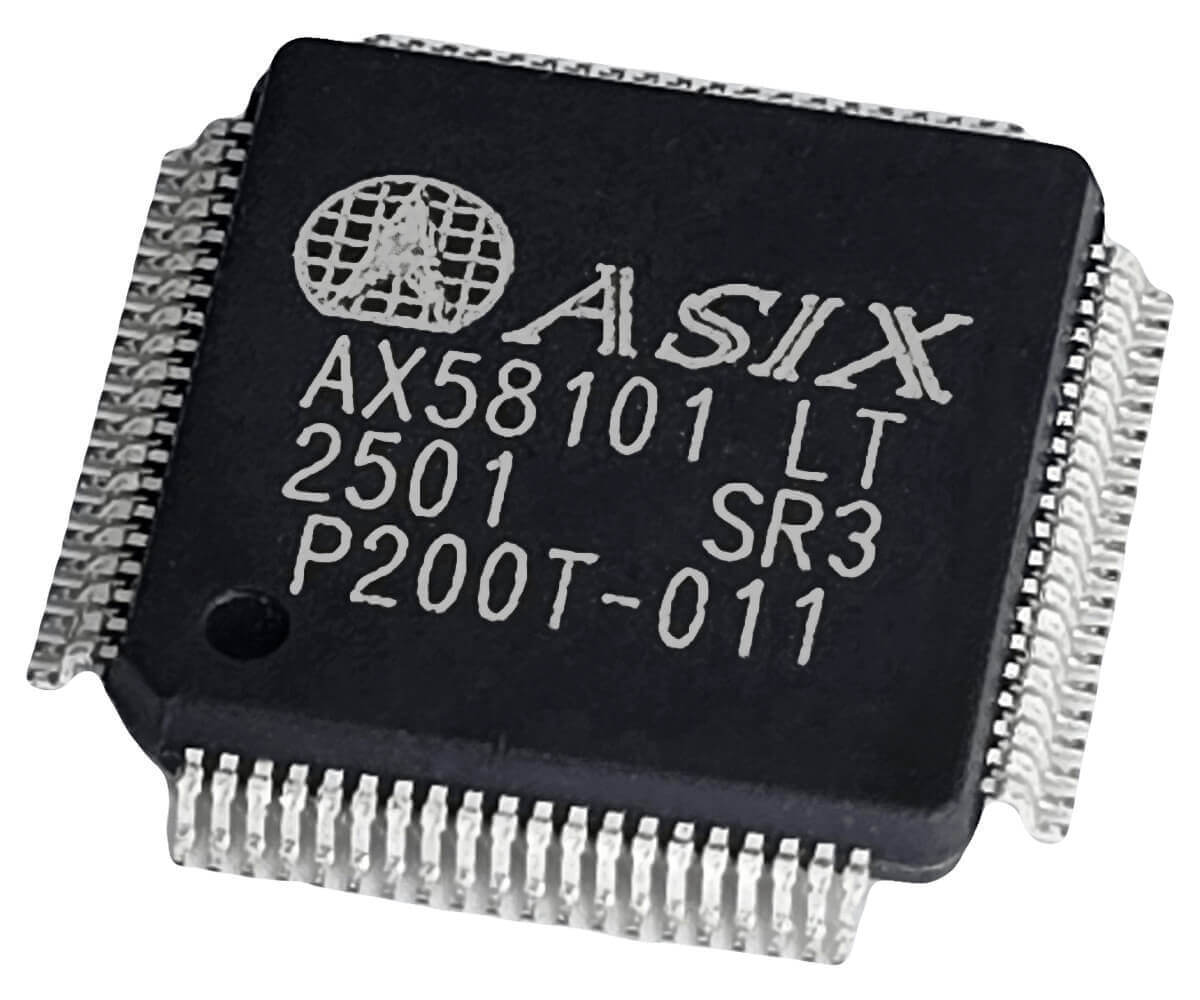
\includegraphics[width=\linewidth]{../figures/d5_ethercat_esc.jpg}
\end{minipage}\hfill
\begin{minipage}[c]{.86\linewidth}
\begin{notebox}
Choose the bus by \hl{cycle time}, \hl{synchronisation accuracy}, number of axes and drive profile, not by raw bit rate. EtherCAT slaves use a dedicated ESC chip (left). Standards: ISO 11898, IEC 61158 / 61784, IEC 61800-7, TIA/EIA-485.
\end{notebox}
\end{minipage}\\
\credit{EtherCAT slave controller IC: Allanchou1357, CC BY-SA 4.0, via Wikimedia Commons}
\end{frame}

% ---------------------------------------------------------------------
\begin{frame}{Latency budget of a distributed position loop}
\centering
\begin{tikzpicture}[font=\tiny]
  \lbx{0}{1.2}{encoder\\sample + link}{mkSky!40}
  \lbx{1.2}{2.4}{drive: wait\\for SYNC}{mkPale}
  \lbx{2.4}{3.6}{bus to\\controller}{mkMid!25}
  \lbx{3.6}{5.4}{controller\\computation}{mkCream}
  \lbx{5.4}{6.6}{bus to\\drive}{mkMid!25}
  \lbx{6.6}{7.8}{apply at\\next SYNC}{mkPale}
  \lbx{7.8}{9.4}{inner loops +\\current response}{mkSky!40}
  \draw[{Latex}-{Latex},mkOrange,thick] (0,-.25) -- (9.4,-.25) node[midway,below]{total dead time $T_d\approx 2$--$3\,T_\text{cyc}$ + inner-loop lag};
\end{tikzpicture}

\vspace{3mm}
\begin{columns}[T]
\column{.5\textwidth}
\begin{keybox}[Worked example]
\footnotesize
$T_\text{cyc}=\SI{250}{\micro s}$, $T_d=2.5\,T_\text{cyc}=\SI{625}{\micro s}$.\\
Position loop in the controller with $f_c=\SI{30}{Hz}$:
$\Delta\varphi=360^\circ\cdot30\cdot625\cdot10^{-6}=6.8^\circ$ --- acceptable.\\
Velocity loop over the bus at $f_c=\SI{200}{Hz}$: $45^\circ$ --- \hl{not acceptable}.
\end{keybox}
\column{.47\textwidth}
\begin{itemize}\footnotesize
\item Close fast loops (current, velocity) \hl{in the drive}; send position set-points (CSP) or velocity set-points (CSV) over the bus.
\item Use velocity / torque \term{feed-forward} values in the PDO to recover dynamics.
\item Time-stamp set-points; interpolate between bus cycles inside the drive.
\end{itemize}
\end{columns}
\end{frame}

% ---------------------------------------------------------------------
\begin{frame}{Data validity: CRC, watchdogs, timestamps}
\begin{columns}[T]
\column{.5\textwidth}
\begin{itemize}\footnotesize
\item \term{CRC}: detects transmission errors (CAN 15 bit, Ethernet FCS CRC-32, encoder CRC 6--16 bit). A CRC-protected value can still be \emph{old}.
\item \term{Working counter / sequence (life) counter}: detects lost, repeated or frozen telegrams.
\item \term{Watchdogs}: SyncManager watchdog (EtherCAT), heartbeat / node guarding (CANopen), software watchdog in the drive firmware.
\item \term{Timestamps}: age of a value $=t_\text{now}-t_\text{sample}$; reject or extrapolate stale data.
\item \term{Plausibility}: range, rate-of-change, cross-checks (two encoders, $i_a+i_b+i_c=0$).
\end{itemize}
\column{.47\textwidth}
\centering
\begin{tikzpicture}[font=\scriptsize,node distance=4mm]
  \node[blk,minimum width=4.4cm] (rx) {telegram received};
  \node[blk,below=of rx,minimum width=4.4cm] (crc) {CRC / WKC ok?};
  \node[blk,below=of crc,minimum width=4.4cm] (seq) {counter advanced, age $<T_\text{max}$?};
  \node[blk,below=of seq,minimum width=4.4cm] (pl) {value plausible?};
  \node[blk,below=of pl,minimum width=4.4cm,fill=mkCream,draw=mkGreen] (use) {use value, reset watchdog};
  \draw[sig] (rx) -- (crc); \draw[sig] (crc) -- (seq); \draw[sig] (seq) -- (pl); \draw[sig] (pl) -- (use);
  \node[blk,right=5mm of seq,fill=mkRed!15,draw=mkRed,minimum width=1.4cm] (err) {hold / ramp\\down, alarm};
  \draw[sig,mkRed] (crc.east) -| (err.north);
  \draw[sig,mkRed] (seq) -- (err);
  \draw[sig,mkRed] (pl.east) -| (err.south);
\end{tikzpicture}

\vspace{1mm}
{\scriptsize Safety functions (STO, SS1, SLS) use a separate \term{black-channel} safety protocol (e.g.\ FSoE, IEC 61784-3) on top of the same bus.}
\end{columns}
\end{frame}

% ---------------------------------------------------------------------
\begin{frame}{Summary: communication and system integration}
\begin{columns}[T]
\column{.55\textwidth}
\begin{itemize}\small
\item CAN/CANopen: robust, deterministic arbitration, $\ge$\SI{1}{ms} cycles.
\item CiA 402 standardises drive state machine, objects and operating modes (CSP/CSV/CST).
\item EtherCAT: on-the-fly processing + distributed clocks $\Rightarrow$ \SI{100}{\micro s} cycles, sub-\si{\micro s} sync.
\item Latency costs phase, jitter costs accuracy: close fast loops locally.
\item Validity needs CRC \emph{and} freshness (counters, watchdogs, timestamps).
\end{itemize}
\column{.42\textwidth}
\begin{keybox}[Integration checklist]
\footnotesize
\checkitem\ cycle time vs.\ loop bandwidths\\
\checkitem\ synchronisation of all sampling\\
\checkitem\ end-to-end latency budget\\
\checkitem\ error reaction for every link\\
\checkitem\ diagnostics and time-stamped logging
\end{keybox}
{\scriptsize\color{mkGray} ETG.1000 / IEC 61158 (EtherCAT); CiA 301, CiA 402; ISO 11898.}
\end{columns}
\end{frame}

% =====================================================================
\section{Day summary and course wrap-up}

\begin{frame}{Day summary}
\begin{columns}[T]
\column{.5\textwidth}
\begin{defbox}[3.7 Resonance]
\footnotesize $\omega_\text{AR}=\sqrt{k/J_L}$, $\omega_\text{R}=\omega_\text{AR}\sqrt{1+R}$; notch for narrow peaks, LPF for broad HF, adaptive notch for drifting modes.
\end{defbox}
\vspace{-1mm}
\begin{defbox}[4.1--4.2 Sensors and position sensing]
\footnotesize Specify accuracy vs.\ resolution; $\times4$ decoding; atan2 interpolation; RDC tracking loop; M/T velocity estimation.
\end{defbox}
\vspace{-1mm}
\begin{defbox}[4.3 Sampling]
\footnotesize SNR $=6.02N+1.76$ dB; alias $=|f-kf_s|$; PWM-synchronous sampling; delay $\to 360^\circ fT_d$.
\end{defbox}
\column{.47\textwidth}
\begin{defbox}[4.4 Filters]
\footnotesize Moving average, FIR vs.\ IIR, Butterworth vs.\ Bessel, filtered derivative, analogue anti-aliasing, biquad DF-II-T.
\end{defbox}
\vspace{-1mm}
\begin{defbox}[4.5 Integration]
\footnotesize CANopen / CiA 402, EtherCAT with DC, latency and jitter budgets, CRC + watchdog + timestamps.
\end{defbox}
\vspace{-1mm}
\begin{keybox}[One sentence]
\footnotesize The achievable servo performance is set by mechanics (resonances) and by the measurement chain (resolution, noise, delay) --- the controller can only use what they allow.
\end{keybox}
\end{columns}
\end{frame}

% ---------------------------------------------------------------------
\begin{frame}{Course wrap-up: five days, one servo axis}
\centering
\begin{tikzpicture}[font=\scriptsize,node distance=5mm,
  day/.style={draw=mkBlue,fill=mkPale,thick,rounded corners=2pt,minimum width=4.5cm,minimum height=9mm,align=left,text width=4.3cm}]
  \node[day] (d1) {\textbf{Day 1} \ Electrical machines \& actuators; intro to modelling};
  \node[day,below=of d1] (d2) {\textbf{Day 2} \ System dynamics, identification, PID, stability};
  \node[day,below=of d2] (d3) {\textbf{Day 3} \ Filters, modern / adaptive / discrete control; servo intro};
  \node[day,below=of d3] (d4) {\textbf{Day 4} \ Drives, FOC, cascaded loops, tuning, compensation};
  \node[day,below=of d4,fill=mkCream,draw=mkOrange] (d5) {\textbf{Day 5} \ Resonance, sensors, sampling, filters, fieldbus};
  % servo loop diagram
  \begin{scope}[xshift=6.6cm,yshift=-2.5cm]
    \node[blk] (pc) at (0,1.6) {position\\controller};
    \node[blk] (vc) at (2.0,1.6) {velocity\\controller};
    \node[blk] (cc) at (4.0,1.6) {current\\(FOC)};
    \node[blk,fill=mkCream,draw=mkOrange] (mo) at (4.0,0) {PMSM +\\mechanics};
    \node[blk,fill=mkSky] (se) at (2.0,0) {sensors\\+ filters};
    \node[blk,fill=mkLight] (fb) at (0,0) {fieldbus};
    \draw[sig] (pc) -- (vc); \draw[sig] (vc) -- (cc); \draw[sig] (cc) -- (mo);
    \draw[sig] (mo) -- (se); \draw[sig] (se) -- (vc); \draw[sig] (se) -- (pc); \draw[sig] (fb) -- (pc);
  \end{scope}
  \foreach \n/\t/\p in {pc/{Days 2, 4}/above,vc/{Days 2--4}/above,cc/{Days 1, 4}/above,mo/{Days 1, 5}/below,se/{Days 3, 5}/below,fb/{Day 5}/below}{
    \node[\p=1mm of \n,font=\tiny\bfseries,text=mkOrange] {\t};}
\end{tikzpicture}
\end{frame}

% ---------------------------------------------------------------------
\begin{frame}{Course wrap-up: ten principles to take home}
\begin{columns}[T]
\column{.5\textwidth}
\begin{enumerate}\footnotesize
\item Know the plant: $R$, $L$, $k_t$, $J$, $B$ and the \hl{mechanics} (Day 1, 5).
\item Model first, then identify and validate with FRFs (Day 2).
\item Loop shaping: $L(s)=C(s)G(s)$, $\omega_c$, PM $\ge 45^\circ$, GM $\ge 6$ dB (Day 2).
\item Every filter and every sample is phase lag (Days 3, 5).
\item Cascade: current $\gg$ velocity $\gg$ position bandwidth, $\times$3--10 per stage (Day 4).
\end{enumerate}
\column{.48\textwidth}
\begin{enumerate}\footnotesize
\setcounter{enumi}{5}
\item Field orientation turns the PMSM into a torque source $T=\tfrac32 p\,\psi_\text{PM}\,i_q$ (Day 4).
\item Feed-forward does the work, feedback fixes the errors (Day 4).
\item Resonances are handled mechanically first, then by notch / LPF (Day 5).
\item Resolution, noise and latency of sensors bound the achievable stiffness (Day 5).
\item Synchronise and time-stamp everything; validate every datum (Day 5).
\end{enumerate}
\end{columns}

\vspace{3mm}
\begin{keybox}[Thank you]
\footnotesize Questions, discussion of your own axes and applications --- and an invitation to measure an FRF on your next machine.
\end{keybox}
\end{frame}

% ---------------------------------------------------------------------
\begin{frame}{Figure credits}
\scriptsize
All plots and diagrams not listed here are original drawings computed for this course (TikZ / pgfplots; data generated by \texttt{day5/data/gen\_data.py}).

\vspace{2mm}
\renewcommand{\arraystretch}{1.15}
\begin{tabularx}{\linewidth}{@{}l X l l@{}}
\toprule
\textbf{File} & \textbf{Wikimedia Commons title} & \textbf{Author} & \textbf{License}\\
\midrule
\texttt{d5\_encoder\_model.jpg} & Encoder.jpg & Rrudzik & CC BY-SA 4.0\\
\texttt{d5\_gray\_encoder.jpg} & Gray code rotary encoder 13-track opened.jpg & Mike1024 & Public domain\\
\texttt{d5\_load\_cell.jpg} & PSCG load cell.jpg & Daraceleste & CC BY-SA 4.0\\
\texttt{d5\_pt100.jpg} & Wire Wound Pt100 Resistor.jpg & Harke & CC BY-SA 3.0\\
\texttt{d5\_thermocouple.jpg} & Thermocouple K (2).jpg & Harke & Public domain\\
\texttt{d5\_hall\_current.jpg} & SparkFun ACS712 HallSensor 08882-01.jpg & SparkFun & CC BY 2.0\\
\texttt{d5\_strain\_gauge.jpg} & Unmounted strain gauge.jpg & Pleriche & CC BY-SA 4.0\\
\texttt{d5\_ethercat\_esc.jpg} & ASIX AX58101 EtherCAT SubDevice Controller.jpg & Allanchou1357 & CC BY-SA 4.0\\
\texttt{d5\_resolver\_principle.png} & ResolverPrinzip.png & Heinz Seehagel (Hasee) & Public domain\\
\texttt{d5\_smd\_shunt.jpg} & SMD Shunt Resistors.jpg & wdwd & CC BY-SA 4.0\\
\bottomrule
\end{tabularx}

\vspace{1mm}
All via Wikimedia Commons (commons.wikimedia.org); licences as stated.
\end{frame}

% ---------------------------------------------------------------------
\begin{frame}{References}
\scriptsize
\begin{itemize}
\item G.~Ellis, \emph{Control System Design Guide}, 4th ed., Butterworth-Heinemann, 2012.
\item G.~F.~Franklin, J.~D.~Powell, A.~Emami-Naeini, \emph{Feedback Control of Dynamic Systems}, 8th ed., Pearson, 2019.
\item G.~F.~Franklin, J.~D.~Powell, M.~L.~Workman, \emph{Digital Control of Dynamic Systems}, 3rd ed., Addison-Wesley, 1998.
\item A.~V.~Oppenheim, R.~W.~Schafer, \emph{Discrete-Time Signal Processing}, 3rd ed., Pearson, 2010.
\item R.~Krishnan, \emph{Permanent Magnet Synchronous and Brushless DC Motor Drives}, CRC Press, 2010.
\item W.~Leonhard, \emph{Control of Electrical Drives}, 3rd ed., Springer, 2001.
\item J.~Fraden, \emph{Handbook of Modern Sensors}, 5th ed., Springer, 2016.
\item K.~J.~\AA{}str\"om, R.~M.~Murray, \emph{Feedback Systems}, 2nd ed., Princeton University Press, 2021.
\item ISO 11898-1/-2 (CAN); CiA 301 and CiA 402 (CANopen, drive profile); IEC 61800-7 (drive profiles).
\item IEC 61158 / IEC 61784 and ETG.1000 (EtherCAT); IEC 60751 (industrial platinum resistance thermometers).
\item Application notes on resolver-to-digital conversion, sigma-delta current sensing and encoder interfaces: Analog Devices, Texas Instruments, Infineon.
\end{itemize}
\end{frame}

\end{document}
